\documentclass{report}

%%%%%%%%%%%%%%%%%%%%%%%%%%%%%%%%%
% PACKAGE IMPORTS
%%%%%%%%%%%%%%%%%%%%%%%%%%%%%%%%%


\usepackage[tmargin=2cm,rmargin=1in,lmargin=1in,margin=0.85in,bmargin=2cm,footskip=.2in]{geometry}
\usepackage{amsmath,amsfonts,amsthm,amssymb,mathtools}
\usepackage[varbb]{newpxmath}
\usepackage{xfrac}
\usepackage[makeroom]{cancel}
\usepackage{mathtools}
\usepackage{bookmark}
\usepackage{enumitem}
\usepackage{listings}
\usepackage{hyperref,theoremref}
\hypersetup{
	pdftitle={Assignment},
	colorlinks=true, linkcolor=myp,
	bookmarksnumbered=true,
	bookmarksopen=true
}
\usepackage[most,many,breakable]{tcolorbox}
\usepackage{xcolor}
\usepackage{varwidth}
\usepackage{varwidth}
\usepackage{etoolbox}
%\usepackage{authblk}
\usepackage{nameref}
\usepackage{multicol,array}
\usepackage{tikz-cd}
\usepackage[ruled,vlined,linesnumbered]{algorithm2e}
\usepackage{comment} % enables the use of multi-line comments (\ifx \fi) 
\usepackage{import}
\usepackage{xifthen}
\usepackage{pdfpages}
\usepackage{transparent}
\usepackage{afterpage}
\usepackage{tikz}
\usetikzlibrary{er, fit}
\usetikzlibrary{positioning}

\newcommand\mycommfont[1]{\footnotesize\ttfamily\textcolor{myp}{#1}}
\SetCommentSty{mycommfont}
\newcommand{\incfig}[1]{%
    \def\svgwidth{\columnwidth}
    \import{./figures/}{#1.pdf_tex}
}

\usepackage{tikzsymbols}
\renewcommand\qedsymbol{$\Laughey$}


%\usepackage{import}
%\usepackage{xifthen}
%\usepackage{pdfpages}
%\usepackage{transparent}

%%%%%%%%%%%%%%%%%%%%%%%%%%%%%%
% BLANK PAGE
%%%%%%%%%%%%%%%%%%%%%%%%%%%%%%

\newcommand\blankpage{%
    \null
    \thispagestyle{empty}%
    \addtocounter{page}{-1}%
    \newpage
}

%%%%%%%%%%%%%%%%%%%%%%%%%%%%%%
% LISTING
%%%%%%%%%%%%%%%%%%%%%%%%%%%%%%

\lstdefinestyle{SQL}{
  language=SQL,
  basicstyle=\ttfamily,
  keywordstyle=\color{blue},
  commentstyle=\color{green},
  stringstyle=\color{red},
  numbers=left,
  numberstyle=\tiny\color{gray},
  stepnumber=1,
  numbersep=5pt,
  breaklines=true,
  showstringspaces=false,
  frame=single,
  captionpos=b
}

%%%%%%%%%%%%%%%%%%%%%%%%%%%%%%
% SELF MADE COLORS
%%%%%%%%%%%%%%%%%%%%%%%%%%%%%%

\definecolor{myg}{RGB}{56, 140, 70}
\definecolor{myb}{RGB}{45, 111, 177}
\definecolor{myr}{RGB}{199, 68, 64}
\definecolor{mytheorembg}{HTML}{F2F2F9}
\definecolor{mytheoremfr}{HTML}{00007B}
\definecolor{mylenmabg}{HTML}{FFFAF8}
\definecolor{mylenmafr}{HTML}{983b0f}
\definecolor{mypropbg}{HTML}{f2fbfc}
\definecolor{mypropfr}{HTML}{191971}
\definecolor{myexamplebg}{HTML}{F2FBF8}
\definecolor{myexamplefr}{HTML}{88D6D1}
\definecolor{myexampleti}{HTML}{2A7F7F}
\definecolor{mydefinitbg}{HTML}{E5E5FF}
\definecolor{mydefinitfr}{HTML}{3F3FA3}
\definecolor{notesred}{RGB}{0,162,0}
\definecolor{myp}{RGB}{197, 92, 212}
\definecolor{mygr}{HTML}{2C3338}
\definecolor{myred}{RGB}{127,0,0}
\definecolor{myyellow}{RGB}{169,121,69}
\definecolor{myexercisebg}{HTML}{F2FBF8}
\definecolor{myexercisefg}{HTML}{88D6D1}

%%%%%%%%%%%%%%%%%%%%%%%%%%%%
% TCOLORBOX SETUPS
%%%%%%%%%%%%%%%%%%%%%%%%%%%%

\setlength{\parindent}{1cm}
%================================
% THEOREM BOX
%================================

\tcbuselibrary{theorems,skins,hooks}
\newtcbtheorem[number within=section]{Theorem}{Teorema}
{%
	enhanced,
	breakable,
	colback = mytheorembg,
	frame hidden,
	boxrule = 0sp,
	borderline west = {2pt}{0pt}{mytheoremfr},
	sharp corners,
	detach title,
	before upper = \tcbtitle\par\smallskip,
	coltitle = mytheoremfr,
	fonttitle = \bfseries\sffamily,
	description font = \mdseries,
	separator sign none,
	segmentation style={solid, mytheoremfr},
}
{th}

\tcbuselibrary{theorems,skins,hooks}
\newtcbtheorem[number within=chapter]{theorem}{Theorem}
{%
	enhanced,
	breakable,
	colback = mytheorembg,
	frame hidden,
	boxrule = 0sp,
	borderline west = {2pt}{0pt}{mytheoremfr},
	sharp corners,
	detach title,
	before upper = \tcbtitle\par\smallskip,
	coltitle = mytheoremfr,
	fonttitle = \bfseries\sffamily,
	description font = \mdseries,
	separator sign none,
	segmentation style={solid, mytheoremfr},
}
{th}


\tcbuselibrary{theorems,skins,hooks}
\newtcolorbox{Theoremcon}
{%
	enhanced
	,breakable
	,colback = mytheorembg
	,frame hidden
	,boxrule = 0sp
	,borderline west = {2pt}{0pt}{mytheoremfr}
	,sharp corners
	,description font = \mdseries
	,separator sign none
}

%================================
% Corollery
%================================
\tcbuselibrary{theorems,skins,hooks}
\newtcbtheorem[number within=section]{Corollary}{Corollary}
{%
	enhanced
	,breakable
	,colback = myp!10
	,frame hidden
	,boxrule = 0sp
	,borderline west = {2pt}{0pt}{myp!85!black}
	,sharp corners
	,detach title
	,before upper = \tcbtitle\par\smallskip
	,coltitle = myp!85!black
	,fonttitle = \bfseries\sffamily
	,description font = \mdseries
	,separator sign none
	,segmentation style={solid, myp!85!black}
}
{th}
\tcbuselibrary{theorems,skins,hooks}
\newtcbtheorem[number within=chapter]{corollary}{Corollary}
{%
	enhanced
	,breakable
	,colback = myp!10
	,frame hidden
	,boxrule = 0sp
	,borderline west = {2pt}{0pt}{myp!85!black}
	,sharp corners
	,detach title
	,before upper = \tcbtitle\par\smallskip
	,coltitle = myp!85!black
	,fonttitle = \bfseries\sffamily
	,description font = \mdseries
	,separator sign none
	,segmentation style={solid, myp!85!black}
}
{th}


%================================
% LENMA
%================================

\tcbuselibrary{theorems,skins,hooks}
\newtcbtheorem[number within=section]{Lenma}{Lenma}
{%
	enhanced,
	breakable,
	colback = mylenmabg,
	frame hidden,
	boxrule = 0sp,
	borderline west = {2pt}{0pt}{mylenmafr},
	sharp corners,
	detach title,
	before upper = \tcbtitle\par\smallskip,
	coltitle = mylenmafr,
	fonttitle = \bfseries\sffamily,
	description font = \mdseries,
	separator sign none,
	segmentation style={solid, mylenmafr},
}
{th}

\tcbuselibrary{theorems,skins,hooks}
\newtcbtheorem[number within=chapter]{lenma}{Lenma}
{%
	enhanced,
	breakable,
	colback = mylenmabg,
	frame hidden,
	boxrule = 0sp,
	borderline west = {2pt}{0pt}{mylenmafr},
	sharp corners,
	detach title,
	before upper = \tcbtitle\par\smallskip,
	coltitle = mylenmafr,
	fonttitle = \bfseries\sffamily,
	description font = \mdseries,
	separator sign none,
	segmentation style={solid, mylenmafr},
}
{th}


%================================
% PROPOSITION
%================================

\tcbuselibrary{theorems,skins,hooks}
\newtcbtheorem[number within=section]{Prop}{Proposition}
{%
	enhanced,
	breakable,
	colback = mypropbg,
	frame hidden,
	boxrule = 0sp,
	borderline west = {2pt}{0pt}{mypropfr},
	sharp corners,
	detach title,
	before upper = \tcbtitle\par\smallskip,
	coltitle = mypropfr,
	fonttitle = \bfseries\sffamily,
	description font = \mdseries,
	separator sign none,
	segmentation style={solid, mypropfr},
}
{th}

\tcbuselibrary{theorems,skins,hooks}
\newtcbtheorem[number within=chapter]{prop}{Proposition}
{%
	enhanced,
	breakable,
	colback = mypropbg,
	frame hidden,
	boxrule = 0sp,
	borderline west = {2pt}{0pt}{mypropfr},
	sharp corners,
	detach title,
	before upper = \tcbtitle\par\smallskip,
	coltitle = mypropfr,
	fonttitle = \bfseries\sffamily,
	description font = \mdseries,
	separator sign none,
	segmentation style={solid, mypropfr},
}
{th}


%================================
% CLAIM
%================================

\tcbuselibrary{theorems,skins,hooks}
\newtcbtheorem[number within=section]{claim}{Claim}
{%
	enhanced
	,breakable
	,colback = myg!10
	,frame hidden
	,boxrule = 0sp
	,borderline west = {2pt}{0pt}{myg}
	,sharp corners
	,detach title
	,before upper = \tcbtitle\par\smallskip
	,coltitle = myg!85!black
	,fonttitle = \bfseries\sffamily
	,description font = \mdseries
	,separator sign none
	,segmentation style={solid, myg!85!black}
}
{th}



%================================
% Exercise
%================================

\tcbuselibrary{theorems,skins,hooks}
\newtcbtheorem[number within=section]{Exercise}{Exercise}
{%
	enhanced,
	breakable,
	colback = myexercisebg,
	frame hidden,
	boxrule = 0sp,
	borderline west = {2pt}{0pt}{myexercisefg},
	sharp corners,
	detach title,
	before upper = \tcbtitle\par\smallskip,
	coltitle = myexercisefg,
	fonttitle = \bfseries\sffamily,
	description font = \mdseries,
	separator sign none,
	segmentation style={solid, myexercisefg},
}
{th}

\tcbuselibrary{theorems,skins,hooks}
\newtcbtheorem[number within=chapter]{exercise}{Exercise}
{%
	enhanced,
	breakable,
	colback = myexercisebg,
	frame hidden,
	boxrule = 0sp,
	borderline west = {2pt}{0pt}{myexercisefg},
	sharp corners,
	detach title,
	before upper = \tcbtitle\par\smallskip,
	coltitle = myexercisefg,
	fonttitle = \bfseries\sffamily,
	description font = \mdseries,
	separator sign none,
	segmentation style={solid, myexercisefg},
}
{th}

%================================
% EXAMPLE BOX
%================================

\newtcbtheorem[number within=section]{Example}{Esempio}
{%
	colback = myexamplebg
	,breakable
	,colframe = myexamplefr
	,coltitle = myexampleti
	,boxrule = 1pt
	,sharp corners
	,detach title
	,before upper=\tcbtitle\par\smallskip
	,fonttitle = \bfseries
	,description font = \mdseries
	,separator sign none
	,description delimiters parenthesis
}
{ex}

\newtcbtheorem[number within=chapter]{example}{Esempio}
{%
	colback = myexamplebg
	,breakable
	,colframe = myexamplefr
	,coltitle = myexampleti
	,boxrule = 1pt
	,sharp corners
	,detach title
	,before upper=\tcbtitle\par\smallskip
	,fonttitle = \bfseries
	,description font = \mdseries
	,separator sign none
	,description delimiters parenthesis
}
{ex}

%================================
% DEFINITION BOX
%================================

\newtcbtheorem[number within=section]{Definizione}{Definizione}{enhanced,
	before skip=2mm,after skip=2mm, colback=red!5,colframe=red!80!black,boxrule=0.5mm,
	attach boxed title to top left={xshift=1cm,yshift*=1mm-\tcboxedtitleheight}, varwidth boxed title*=-3cm,
	boxed title style={frame code={
					\path[fill=tcbcolback]
					([yshift=-1mm,xshift=-1mm]frame.north west)
					arc[start angle=0,end angle=180,radius=1mm]
					([yshift=-1mm,xshift=1mm]frame.north east)
					arc[start angle=180,end angle=0,radius=1mm];
					\path[left color=tcbcolback!60!black,right color=tcbcolback!60!black,
						middle color=tcbcolback!80!black]
					([xshift=-2mm]frame.north west) -- ([xshift=2mm]frame.north east)
					[rounded corners=1mm]-- ([xshift=1mm,yshift=-1mm]frame.north east)
					-- (frame.south east) -- (frame.south west)
					-- ([xshift=-1mm,yshift=-1mm]frame.north west)
					[sharp corners]-- cycle;
				},interior engine=empty,
		},
	fonttitle=\bfseries,
	title={#2},#1}{def}
\newtcbtheorem[number within=chapter]{definizione}{Definizione}{enhanced,
	before skip=2mm,after skip=2mm, colback=red!5,colframe=red!80!black,boxrule=0.5mm,
	attach boxed title to top left={xshift=1cm,yshift*=1mm-\tcboxedtitleheight}, varwidth boxed title*=-3cm,
	boxed title style={frame code={
					\path[fill=tcbcolback]
					([yshift=-1mm,xshift=-1mm]frame.north west)
					arc[start angle=0,end angle=180,radius=1mm]
					([yshift=-1mm,xshift=1mm]frame.north east)
					arc[start angle=180,end angle=0,radius=1mm];
					\path[left color=tcbcolback!60!black,right color=tcbcolback!60!black,
						middle color=tcbcolback!80!black]
					([xshift=-2mm]frame.north west) -- ([xshift=2mm]frame.north east)
					[rounded corners=1mm]-- ([xshift=1mm,yshift=-1mm]frame.north east)
					-- (frame.south east) -- (frame.south west)
					-- ([xshift=-1mm,yshift=-1mm]frame.north west)
					[sharp corners]-- cycle;
				},interior engine=empty,
		},
	fonttitle=\bfseries,
	title={#2},#1}{def}



%================================
% Solution BOX
%================================

\makeatletter
\newtcbtheorem{question}{Question}{enhanced,
	breakable,
	colback=white,
	colframe=myb!80!black,
	attach boxed title to top left={yshift*=-\tcboxedtitleheight},
	fonttitle=\bfseries,
	title={#2},
	boxed title size=title,
	boxed title style={%
			sharp corners,
			rounded corners=northwest,
			colback=tcbcolframe,
			boxrule=0pt,
		},
	underlay boxed title={%
			\path[fill=tcbcolframe] (title.south west)--(title.south east)
			to[out=0, in=180] ([xshift=5mm]title.east)--
			(title.center-|frame.east)
			[rounded corners=\kvtcb@arc] |-
			(frame.north) -| cycle;
		},
	#1
}{def}
\makeatother

%================================
% SOLUTION BOX
%================================

\makeatletter
\newtcolorbox{solution}{enhanced,
	breakable,
	colback=white,
	colframe=myg!80!black,
	attach boxed title to top left={yshift*=-\tcboxedtitleheight},
	title=Solution,
	boxed title size=title,
	boxed title style={%
			sharp corners,
			rounded corners=northwest,
			colback=tcbcolframe,
			boxrule=0pt,
		},
	underlay boxed title={%
			\path[fill=tcbcolframe] (title.south west)--(title.south east)
			to[out=0, in=180] ([xshift=5mm]title.east)--
			(title.center-|frame.east)
			[rounded corners=\kvtcb@arc] |-
			(frame.north) -| cycle;
		},
}
\makeatother

%================================
% Question BOX
%================================

\makeatletter
\newtcbtheorem{qstion}{Question}{enhanced,
	breakable,
	colback=white,
	colframe=mygr,
	attach boxed title to top left={yshift*=-\tcboxedtitleheight},
	fonttitle=\bfseries,
	title={#2},
	boxed title size=title,
	boxed title style={%
			sharp corners,
			rounded corners=northwest,
			colback=tcbcolframe,
			boxrule=0pt,
		},
	underlay boxed title={%
			\path[fill=tcbcolframe] (title.south west)--(title.south east)
			to[out=0, in=180] ([xshift=5mm]title.east)--
			(title.center-|frame.east)
			[rounded corners=\kvtcb@arc] |-
			(frame.north) -| cycle;
		},
	#1
}{def}
\makeatother

\newtcbtheorem[number within=chapter]{wconc}{Wrong Concept}{
	breakable,
	enhanced,
	colback=white,
	colframe=myr,
	arc=0pt,
	outer arc=0pt,
	fonttitle=\bfseries\sffamily\large,
	colbacktitle=myr,
	attach boxed title to top left={},
	boxed title style={
			enhanced,
			skin=enhancedfirst jigsaw,
			arc=3pt,
			bottom=0pt,
			interior style={fill=myr}
		},
	#1
}{def}



%================================
% NOTE BOX
%================================

\usetikzlibrary{arrows,calc,shadows.blur}
\tcbuselibrary{skins}
\newtcolorbox{note}[1][]{%
	enhanced jigsaw,
	colback=gray!20!white,%
	colframe=gray!80!black,
	size=small,
	boxrule=1pt,
	title=\textbf{Note:-},
	halign title=flush center,
	coltitle=black,
	breakable,
	drop shadow=black!50!white,
	attach boxed title to top left={xshift=1cm,yshift=-\tcboxedtitleheight/2,yshifttext=-\tcboxedtitleheight/2},
	minipage boxed title=1.5cm,
	boxed title style={%
			colback=white,
			size=fbox,
			boxrule=1pt,
			boxsep=2pt,
			underlay={%
					\coordinate (dotA) at ($(interior.west) + (-0.5pt,0)$);
					\coordinate (dotB) at ($(interior.east) + (0.5pt,0)$);
					\begin{scope}
						\clip (interior.north west) rectangle ([xshift=3ex]interior.east);
						\filldraw [white, blur shadow={shadow opacity=60, shadow yshift=-.75ex}, rounded corners=2pt] (interior.north west) rectangle (interior.south east);
					\end{scope}
					\begin{scope}[gray!80!black]
						\fill (dotA) circle (2pt);
						\fill (dotB) circle (2pt);
					\end{scope}
				},
		},
	#1,
}

%%%%%%%%%%%%%%%%%%%%%%%%%%%%%%
% SELF MADE COMMANDS
%%%%%%%%%%%%%%%%%%%%%%%%%%%%%%


\newcommand{\thm}[2]{\begin{Theorem}{#1}{}#2\end{Theorem}}
\newcommand{\cor}[2]{\begin{Corollary}{#1}{}#2\end{Corollary}}
\newcommand{\mlenma}[2]{\begin{Lenma}{#1}{}#2\end{Lenma}}
\newcommand{\mprop}[2]{\begin{Prop}{#1}{}#2\end{Prop}}
\newcommand{\clm}[3]{\begin{claim}{#1}{#2}#3\end{claim}}
\newcommand{\wc}[2]{\begin{wconc}{#1}{}\setlength{\parindent}{1cm}#2\end{wconc}}
\newcommand{\thmcon}[1]{\begin{Theoremcon}{#1}\end{Theoremcon}}
\newcommand{\ex}[2]{\begin{Example}{#1}{}#2\end{Example}}
\newcommand{\dfn}[2]{\begin{Definizione}[colbacktitle=red!75!black]{#1}{}#2\end{Definizione}}
\newcommand{\dfnc}[2]{\begin{definizione}[colbacktitle=red!75!black]{#1}{}#2\end{definizione}}
\newcommand{\qs}[2]{\begin{question}{#1}{}#2\end{question}}
\newcommand{\pf}[2]{\begin{myproof}[#1]#2\end{myproof}}
\newcommand{\nt}[1]{\begin{note}#1\end{note}}

\newcommand*\circled[1]{\tikz[baseline=(char.base)]{
		\node[shape=circle,draw,inner sep=1pt] (char) {#1};}}
\newcommand\getcurrentref[1]{%
	\ifnumequal{\value{#1}}{0}
	{??}
	{\the\value{#1}}%
}
\newcommand{\getCurrentSectionNumber}{\getcurrentref{section}}
\newenvironment{myproof}[1][\proofname]{%
	\proof[\bfseries #1: ]%
}{\endproof}

\newcommand{\mclm}[2]{\begin{myclaim}[#1]#2\end{myclaim}}
\newenvironment{myclaim}[1][\claimname]{\proof[\bfseries #1: ]}{}

\newcounter{mylabelcounter}

\makeatletter
\newcommand{\setword}[2]{%
	\phantomsection
	#1\def\@currentlabel{\unexpanded{#1}}\label{#2}%
}
\makeatother




\tikzset{
	symbol/.style={
			draw=none,
			every to/.append style={
					edge node={node [sloped, allow upside down, auto=false]{$#1$}}}
		}
}


% deliminators
\DeclarePairedDelimiter{\abs}{\lvert}{\rvert}
\DeclarePairedDelimiter{\norm}{\lVert}{\rVert}

\DeclarePairedDelimiter{\ceil}{\lceil}{\rceil}
\DeclarePairedDelimiter{\floor}{\lfloor}{\rfloor}
\DeclarePairedDelimiter{\round}{\lfloor}{\rceil}

\newsavebox\diffdbox
\newcommand{\slantedromand}{{\mathpalette\makesl{d}}}
\newcommand{\makesl}[2]{%
\begingroup
\sbox{\diffdbox}{$\mathsurround=0pt#1\mathrm{#2}$}%
\pdfsave
\pdfsetmatrix{1 0 0.2 1}%
\rlap{\usebox{\diffdbox}}%
\pdfrestore
\hskip\wd\diffdbox
\endgroup
}
\newcommand{\dd}[1][]{\ensuremath{\mathop{}\!\ifstrempty{#1}{%
\slantedromand\@ifnextchar^{\hspace{0.2ex}}{\hspace{0.1ex}}}%
{\slantedromand\hspace{0.2ex}^{#1}}}}
\ProvideDocumentCommand\dv{o m g}{%
  \ensuremath{%
    \IfValueTF{#3}{%
      \IfNoValueTF{#1}{%
        \frac{\dd #2}{\dd #3}%
      }{%
        \frac{\dd^{#1} #2}{\dd #3^{#1}}%
      }%
    }{%
      \IfNoValueTF{#1}{%
        \frac{\dd}{\dd #2}%
      }{%
        \frac{\dd^{#1}}{\dd #2^{#1}}%
      }%
    }%
  }%
}
\providecommand*{\pdv}[3][]{\frac{\partial^{#1}#2}{\partial#3^{#1}}}
%  - others
\DeclareMathOperator{\Lap}{\mathcal{L}}
\DeclareMathOperator{\Var}{Var} % varience
\DeclareMathOperator{\Cov}{Cov} % covarience
\DeclareMathOperator{\E}{E} % expected

% Since the amsthm package isn't loaded

% I prefer the slanted \leq
\let\oldleq\leq % save them in case they're every wanted
\let\oldgeq\geq
\renewcommand{\leq}{\leqslant}
\renewcommand{\geq}{\geqslant}

% % redefine matrix env to allow for alignment, use r as default
% \renewcommand*\env@matrix[1][r]{\hskip -\arraycolsep
%     \let\@ifnextchar\new@ifnextchar
%     \array{*\c@MaxMatrixCols #1}}


%\usepackage{framed}
%\usepackage{titletoc}
%\usepackage{etoolbox}
%\usepackage{lmodern}


%\patchcmd{\tableofcontents}{\contentsname}{\sffamily\contentsname}{}{}

%\renewenvironment{leftbar}
%{\def\FrameCommand{\hspace{6em}%
%		{\color{myyellow}\vrule width 2pt depth 6pt}\hspace{1em}}%
%	\MakeFramed{\parshape 1 0cm \dimexpr\textwidth-6em\relax\FrameRestore}\vskip2pt%
%}
%{\endMakeFramed}

%\titlecontents{chapter}
%[0em]{\vspace*{2\baselineskip}}
%{\parbox{4.5em}{%
%		\hfill\Huge\sffamily\bfseries\color{myred}\thecontentspage}%
%	\vspace*{-2.3\baselineskip}\leftbar\textsc{\small\chaptername~\thecontentslabel}\\\sffamily}
%{}{\endleftbar}
%\titlecontents{section}
%[8.4em]
%{\sffamily\contentslabel{3em}}{}{}
%{\hspace{0.5em}\nobreak\itshape\color{myred}\contentspage}
%\titlecontents{subsection}
%[8.4em]
%{\sffamily\contentslabel{3em}}{}{}  
%{\hspace{0.5em}\nobreak\itshape\color{myred}\contentspage}



%%%%%%%%%%%%%%%%%%%%%%%%%%%%%%%%%%%%%%%%%%%
% TABLE OF CONTENTS
%%%%%%%%%%%%%%%%%%%%%%%%%%%%%%%%%%%%%%%%%%%

\usepackage{tikz}
\definecolor{doc}{RGB}{0,60,110}
\usepackage{titletoc}
\contentsmargin{0cm}
\titlecontents{chapter}[3.7pc]
{\addvspace{30pt}%
	\begin{tikzpicture}[remember picture, overlay]%
		\draw[fill=myp,draw=myp] (-7.3,-.1) rectangle (-0.9,.5);%
		\pgftext[left,x=-3.7cm,y=0.2cm]{\color{white}\Large\sc\bfseries Capitolo\ \thecontentslabel};%
	\end{tikzpicture}\color{myp}\large\sc\bfseries}%
{}
{}
{\;\titlerule\;\large\sc\bfseries Pagina \thecontentspage
	\begin{tikzpicture}[remember picture, overlay]
		\draw[fill=myp,draw=myp] (2pt,0) rectangle (4,0.1pt);
	\end{tikzpicture}}%
\titlecontents{section}[3.7pc]
{\addvspace{2pt}}
{\contentslabel[\thecontentslabel]{2pc}}
{}
{\hfill\small \thecontentspage}
[]
\titlecontents*{subsection}[3.7pc]
{\addvspace{-1pt}\small}
{}
{}
{\ --- \small\thecontentspage}
[ \textbullet\ ][]

\makeatletter
\renewcommand{\chaptername}{Capitolo}
\renewcommand{\tableofcontents}{%
	\chapter*{%
	  \vspace*{-20\p@}%
	  \begin{tikzpicture}[remember picture, overlay]%
		  \pgftext[right,x=15cm,y=0.2cm]{\color{myp}\Huge\sc\bfseries \contentsname};%
		  \draw[fill=myp,draw=myp] (13,-.75) rectangle (20,1);%
		  \clip (13,-.75) rectangle (20,1);
		  \pgftext[right,x=15cm,y=0.2cm]{\color{white}\Huge\sc\bfseries \contentsname};%
	  \end{tikzpicture}}%
	\@starttoc{toc}}
\makeatother

%%%%%%%%%%%%%%%%%%%%%%%%%%%%%%%%%%%%%%%%%%%
% HYPERLINK
%%%%%%%%%%%%%%%%%%%%%%%%%%%%%%%%%%%%%%%%%%%

\hypersetup{
    colorlinks,
    citecolor=black,
    filecolor=black,
    linkcolor=black,
    urlcolor=black
}
%From M275 "Topology" at SJSU
\newcommand{\id}{\mathrm{id}}
\newcommand{\taking}[1]{\xrightarrow{#1}}
\newcommand{\inv}{^{-1}}

%From M170 "Introduction to Graph Theory" at SJSU
\DeclareMathOperator{\diam}{diam}
\DeclareMathOperator{\ord}{ord}
\newcommand{\defeq}{\overset{\mathrm{def}}{=}}

%From the USAMO .tex files
\newcommand{\ts}{\textsuperscript}
\newcommand{\dg}{^\circ}
\newcommand{\ii}{\item}

% % From Math 55 and Math 145 at Harvard
% \newenvironment{subproof}[1][Proof]{%
% \begin{proof}[#1] \renewcommand{\qedsymbol}{$\blacksquare$}}%
% {\end{proof}}

\newcommand{\liff}{\leftrightarrow}
\newcommand{\lthen}{\rightarrow}
\newcommand{\opname}{\operatorname}
\newcommand{\surjto}{\twoheadrightarrow}
\newcommand{\injto}{\hookrightarrow}
\newcommand{\On}{\mathrm{On}} % ordinals
\DeclareMathOperator{\img}{im} % Image
\DeclareMathOperator{\Img}{Im} % Image
\DeclareMathOperator{\coker}{coker} % Cokernel
\DeclareMathOperator{\Coker}{Coker} % Cokernel
\DeclareMathOperator{\Ker}{Ker} % Kernel
\DeclareMathOperator{\rank}{rank}
\DeclareMathOperator{\Spec}{Spec} % spectrum
\DeclareMathOperator{\Tr}{Tr} % trace
\DeclareMathOperator{\pr}{pr} % projection
\DeclareMathOperator{\ext}{ext} % extension
\DeclareMathOperator{\pred}{pred} % predecessor
\DeclareMathOperator{\dom}{dom} % domain
\DeclareMathOperator{\ran}{ran} % range
\DeclareMathOperator{\Hom}{Hom} % homomorphism
\DeclareMathOperator{\Mor}{Mor} % morphisms
\DeclareMathOperator{\End}{End} % endomorphism

\newcommand{\eps}{\epsilon}
\newcommand{\veps}{\varepsilon}
\newcommand{\ol}{\overline}
\newcommand{\ul}{\underline}
\newcommand{\wt}{\widetilde}
\newcommand{\wh}{\widehat}
\newcommand{\vocab}[1]{\textbf{\color{blue} #1}}
\providecommand{\half}{\frac{1}{2}}
\newcommand{\dang}{\measuredangle} %% Directed angle
\newcommand{\ray}[1]{\overrightarrow{#1}}
\newcommand{\seg}[1]{\overline{#1}}
\newcommand{\arc}[1]{\wideparen{#1}}
\DeclareMathOperator{\cis}{cis}
\DeclareMathOperator*{\lcm}{lcm}
\DeclareMathOperator*{\argmin}{arg min}
\DeclareMathOperator*{\argmax}{arg max}
\newcommand{\cycsum}{\sum_{\mathrm{cyc}}}
\newcommand{\symsum}{\sum_{\mathrm{sym}}}
\newcommand{\cycprod}{\prod_{\mathrm{cyc}}}
\newcommand{\symprod}{\prod_{\mathrm{sym}}}
\newcommand{\Qed}{\begin{flushright}\qed\end{flushright}}
\newcommand{\parinn}{\setlength{\parindent}{1cm}}
\newcommand{\parinf}{\setlength{\parindent}{0cm}}
% \newcommand{\norm}{\|\cdot\|}
\newcommand{\inorm}{\norm_{\infty}}
\newcommand{\opensets}{\{V_{\alpha}\}_{\alpha\in I}}
\newcommand{\oset}{V_{\alpha}}
\newcommand{\opset}[1]{V_{\alpha_{#1}}}
\newcommand{\lub}{\text{lub}}
\newcommand{\del}[2]{\frac{\partial #1}{\partial #2}}
\newcommand{\Del}[3]{\frac{\partial^{#1} #2}{\partial^{#1} #3}}
\newcommand{\deld}[2]{\dfrac{\partial #1}{\partial #2}}
\newcommand{\Deld}[3]{\dfrac{\partial^{#1} #2}{\partial^{#1} #3}}
\newcommand{\lm}{\lambda}
\newcommand{\uin}{\mathbin{\rotatebox[origin=c]{90}{$\in$}}}
\newcommand{\usubset}{\mathbin{\rotatebox[origin=c]{90}{$\subset$}}}
\newcommand{\lt}{\left}
\newcommand{\rt}{\right}
\newcommand{\bs}[1]{\boldsymbol{#1}}
\newcommand{\exs}{\exists}
\newcommand{\st}{\strut}
\newcommand{\dps}[1]{\displaystyle{#1}}

\newcommand{\sol}{\setlength{\parindent}{0cm}\textbf{\textit{Solution:}}\setlength{\parindent}{1cm} }
\newcommand{\solve}[1]{\setlength{\parindent}{0cm}\textbf{\textit{Solution: }}\setlength{\parindent}{1cm}#1 \Qed}
% Things Lie
\newcommand{\kb}{\mathfrak b}
\newcommand{\kg}{\mathfrak g}
\newcommand{\kh}{\mathfrak h}
\newcommand{\kn}{\mathfrak n}
\newcommand{\ku}{\mathfrak u}
\newcommand{\kz}{\mathfrak z}
\DeclareMathOperator{\Ext}{Ext} % Ext functor
\DeclareMathOperator{\Tor}{Tor} % Tor functor
\newcommand{\gl}{\opname{\mathfrak{gl}}} % frak gl group
\renewcommand{\sl}{\opname{\mathfrak{sl}}} % frak sl group chktex 6

% More script letters etc.
\newcommand{\SA}{\mathcal A}
\newcommand{\SB}{\mathcal B}
\newcommand{\SC}{\mathcal C}
\newcommand{\SF}{\mathcal F}
\newcommand{\SG}{\mathcal G}
\newcommand{\SH}{\mathcal H}
\newcommand{\OO}{\mathcal O}

\newcommand{\SCA}{\mathscr A}
\newcommand{\SCB}{\mathscr B}
\newcommand{\SCC}{\mathscr C}
\newcommand{\SCD}{\mathscr D}
\newcommand{\SCE}{\mathscr E}
\newcommand{\SCF}{\mathscr F}
\newcommand{\SCG}{\mathscr G}
\newcommand{\SCH}{\mathscr H}

% Mathfrak primes
\newcommand{\km}{\mathfrak m}
\newcommand{\kp}{\mathfrak p}
\newcommand{\kq}{\mathfrak q}

% number sets
\newcommand{\RR}[1][]{\ensuremath{\ifstrempty{#1}{\mathbb{R}}{\mathbb{R}^{#1}}}}
\newcommand{\NN}[1][]{\ensuremath{\ifstrempty{#1}{\mathbb{N}}{\mathbb{N}^{#1}}}}
\newcommand{\ZZ}[1][]{\ensuremath{\ifstrempty{#1}{\mathbb{Z}}{\mathbb{Z}^{#1}}}}
\newcommand{\QQ}[1][]{\ensuremath{\ifstrempty{#1}{\mathbb{Q}}{\mathbb{Q}^{#1}}}}
\newcommand{\CC}[1][]{\ensuremath{\ifstrempty{#1}{\mathbb{C}}{\mathbb{C}^{#1}}}}
\newcommand{\PP}[1][]{\ensuremath{\ifstrempty{#1}{\mathbb{P}}{\mathbb{P}^{#1}}}}
\newcommand{\HH}[1][]{\ensuremath{\ifstrempty{#1}{\mathbb{H}}{\mathbb{H}^{#1}}}}
\newcommand{\FF}[1][]{\ensuremath{\ifstrempty{#1}{\mathbb{F}}{\mathbb{F}^{#1}}}}
% expected value
\newcommand{\EE}{\ensuremath{\mathbb{E}}}
\newcommand{\charin}{\text{ char }}
\DeclareMathOperator{\sign}{sign}
\DeclareMathOperator{\Aut}{Aut}
\DeclareMathOperator{\Inn}{Inn}
\DeclareMathOperator{\Syl}{Syl}
\DeclareMathOperator{\Gal}{Gal}
\DeclareMathOperator{\GL}{GL} % General linear group
\DeclareMathOperator{\SL}{SL} % Special linear group

%---------------------------------------
% BlackBoard Math Fonts :-
%---------------------------------------

%Captital Letters
\newcommand{\bbA}{\mathbb{A}}	\newcommand{\bbB}{\mathbb{B}}
\newcommand{\bbC}{\mathbb{C}}	\newcommand{\bbD}{\mathbb{D}}
\newcommand{\bbE}{\mathbb{E}}	\newcommand{\bbF}{\mathbb{F}}
\newcommand{\bbG}{\mathbb{G}}	\newcommand{\bbH}{\mathbb{H}}
\newcommand{\bbI}{\mathbb{I}}	\newcommand{\bbJ}{\mathbb{J}}
\newcommand{\bbK}{\mathbb{K}}	\newcommand{\bbL}{\mathbb{L}}
\newcommand{\bbM}{\mathbb{M}}	\newcommand{\bbN}{\mathbb{N}}
\newcommand{\bbO}{\mathbb{O}}	\newcommand{\bbP}{\mathbb{P}}
\newcommand{\bbQ}{\mathbb{Q}}	\newcommand{\bbR}{\mathbb{R}}
\newcommand{\bbS}{\mathbb{S}}	\newcommand{\bbT}{\mathbb{T}}
\newcommand{\bbU}{\mathbb{U}}	\newcommand{\bbV}{\mathbb{V}}
\newcommand{\bbW}{\mathbb{W}}	\newcommand{\bbX}{\mathbb{X}}
\newcommand{\bbY}{\mathbb{Y}}	\newcommand{\bbZ}{\mathbb{Z}}

%---------------------------------------
% MathCal Fonts :-
%---------------------------------------

%Captital Letters
\newcommand{\mcA}{\mathcal{A}}	\newcommand{\mcB}{\mathcal{B}}
\newcommand{\mcC}{\mathcal{C}}	\newcommand{\mcD}{\mathcal{D}}
\newcommand{\mcE}{\mathcal{E}}	\newcommand{\mcF}{\mathcal{F}}
\newcommand{\mcG}{\mathcal{G}}	\newcommand{\mcH}{\mathcal{H}}
\newcommand{\mcI}{\mathcal{I}}	\newcommand{\mcJ}{\mathcal{J}}
\newcommand{\mcK}{\mathcal{K}}	\newcommand{\mcL}{\mathcal{L}}
\newcommand{\mcM}{\mathcal{M}}	\newcommand{\mcN}{\mathcal{N}}
\newcommand{\mcO}{\mathcal{O}}	\newcommand{\mcP}{\mathcal{P}}
\newcommand{\mcQ}{\mathcal{Q}}	\newcommand{\mcR}{\mathcal{R}}
\newcommand{\mcS}{\mathcal{S}}	\newcommand{\mcT}{\mathcal{T}}
\newcommand{\mcU}{\mathcal{U}}	\newcommand{\mcV}{\mathcal{V}}
\newcommand{\mcW}{\mathcal{W}}	\newcommand{\mcX}{\mathcal{X}}
\newcommand{\mcY}{\mathcal{Y}}	\newcommand{\mcZ}{\mathcal{Z}}


%---------------------------------------
% Bold Math Fonts :-
%---------------------------------------

%Captital Letters
\newcommand{\bmA}{\boldsymbol{A}}	\newcommand{\bmB}{\boldsymbol{B}}
\newcommand{\bmC}{\boldsymbol{C}}	\newcommand{\bmD}{\boldsymbol{D}}
\newcommand{\bmE}{\boldsymbol{E}}	\newcommand{\bmF}{\boldsymbol{F}}
\newcommand{\bmG}{\boldsymbol{G}}	\newcommand{\bmH}{\boldsymbol{H}}
\newcommand{\bmI}{\boldsymbol{I}}	\newcommand{\bmJ}{\boldsymbol{J}}
\newcommand{\bmK}{\boldsymbol{K}}	\newcommand{\bmL}{\boldsymbol{L}}
\newcommand{\bmM}{\boldsymbol{M}}	\newcommand{\bmN}{\boldsymbol{N}}
\newcommand{\bmO}{\boldsymbol{O}}	\newcommand{\bmP}{\boldsymbol{P}}
\newcommand{\bmQ}{\boldsymbol{Q}}	\newcommand{\bmR}{\boldsymbol{R}}
\newcommand{\bmS}{\boldsymbol{S}}	\newcommand{\bmT}{\boldsymbol{T}}
\newcommand{\bmU}{\boldsymbol{U}}	\newcommand{\bmV}{\boldsymbol{V}}
\newcommand{\bmW}{\boldsymbol{W}}	\newcommand{\bmX}{\boldsymbol{X}}
\newcommand{\bmY}{\boldsymbol{Y}}	\newcommand{\bmZ}{\boldsymbol{Z}}
%Small Letters
\newcommand{\bma}{\boldsymbol{a}}	\newcommand{\bmb}{\boldsymbol{b}}
\newcommand{\bmc}{\boldsymbol{c}}	\newcommand{\bmd}{\boldsymbol{d}}
\newcommand{\bme}{\boldsymbol{e}}	\newcommand{\bmf}{\boldsymbol{f}}
\newcommand{\bmg}{\boldsymbol{g}}	\newcommand{\bmh}{\boldsymbol{h}}
\newcommand{\bmi}{\boldsymbol{i}}	\newcommand{\bmj}{\boldsymbol{j}}
\newcommand{\bmk}{\boldsymbol{k}}	\newcommand{\bml}{\boldsymbol{l}}
\newcommand{\bmm}{\boldsymbol{m}}	\newcommand{\bmn}{\boldsymbol{n}}
\newcommand{\bmo}{\boldsymbol{o}}	\newcommand{\bmp}{\boldsymbol{p}}
\newcommand{\bmq}{\boldsymbol{q}}	\newcommand{\bmr}{\boldsymbol{r}}
\newcommand{\bms}{\boldsymbol{s}}	\newcommand{\bmt}{\boldsymbol{t}}
\newcommand{\bmu}{\boldsymbol{u}}	\newcommand{\bmv}{\boldsymbol{v}}
\newcommand{\bmw}{\boldsymbol{w}}	\newcommand{\bmx}{\boldsymbol{x}}
\newcommand{\bmy}{\boldsymbol{y}}	\newcommand{\bmz}{\boldsymbol{z}}

%---------------------------------------
% Scr Math Fonts :-
%---------------------------------------

\newcommand{\sA}{{\mathscr{A}}}   \newcommand{\sB}{{\mathscr{B}}}
\newcommand{\sC}{{\mathscr{C}}}   \newcommand{\sD}{{\mathscr{D}}}
\newcommand{\sE}{{\mathscr{E}}}   \newcommand{\sF}{{\mathscr{F}}}
\newcommand{\sG}{{\mathscr{G}}}   \newcommand{\sH}{{\mathscr{H}}}
\newcommand{\sI}{{\mathscr{I}}}   \newcommand{\sJ}{{\mathscr{J}}}
\newcommand{\sK}{{\mathscr{K}}}   \newcommand{\sL}{{\mathscr{L}}}
\newcommand{\sM}{{\mathscr{M}}}   \newcommand{\sN}{{\mathscr{N}}}
\newcommand{\sO}{{\mathscr{O}}}   \newcommand{\sP}{{\mathscr{P}}}
\newcommand{\sQ}{{\mathscr{Q}}}   \newcommand{\sR}{{\mathscr{R}}}
\newcommand{\sS}{{\mathscr{S}}}   \newcommand{\sT}{{\mathscr{T}}}
\newcommand{\sU}{{\mathscr{U}}}   \newcommand{\sV}{{\mathscr{V}}}
\newcommand{\sW}{{\mathscr{W}}}   \newcommand{\sX}{{\mathscr{X}}}
\newcommand{\sY}{{\mathscr{Y}}}   \newcommand{\sZ}{{\mathscr{Z}}}


%---------------------------------------
% Math Fraktur Font
%---------------------------------------

%Captital Letters
\newcommand{\mfA}{\mathfrak{A}}	\newcommand{\mfB}{\mathfrak{B}}
\newcommand{\mfC}{\mathfrak{C}}	\newcommand{\mfD}{\mathfrak{D}}
\newcommand{\mfE}{\mathfrak{E}}	\newcommand{\mfF}{\mathfrak{F}}
\newcommand{\mfG}{\mathfrak{G}}	\newcommand{\mfH}{\mathfrak{H}}
\newcommand{\mfI}{\mathfrak{I}}	\newcommand{\mfJ}{\mathfrak{J}}
\newcommand{\mfK}{\mathfrak{K}}	\newcommand{\mfL}{\mathfrak{L}}
\newcommand{\mfM}{\mathfrak{M}}	\newcommand{\mfN}{\mathfrak{N}}
\newcommand{\mfO}{\mathfrak{O}}	\newcommand{\mfP}{\mathfrak{P}}
\newcommand{\mfQ}{\mathfrak{Q}}	\newcommand{\mfR}{\mathfrak{R}}
\newcommand{\mfS}{\mathfrak{S}}	\newcommand{\mfT}{\mathfrak{T}}
\newcommand{\mfU}{\mathfrak{U}}	\newcommand{\mfV}{\mathfrak{V}}
\newcommand{\mfW}{\mathfrak{W}}	\newcommand{\mfX}{\mathfrak{X}}
\newcommand{\mfY}{\mathfrak{Y}}	\newcommand{\mfZ}{\mathfrak{Z}}
%Small Letters
\newcommand{\mfa}{\mathfrak{a}}	\newcommand{\mfb}{\mathfrak{b}}
\newcommand{\mfc}{\mathfrak{c}}	\newcommand{\mfd}{\mathfrak{d}}
\newcommand{\mfe}{\mathfrak{e}}	\newcommand{\mff}{\mathfrak{f}}
\newcommand{\mfg}{\mathfrak{g}}	\newcommand{\mfh}{\mathfrak{h}}
\newcommand{\mfi}{\mathfrak{i}}	\newcommand{\mfj}{\mathfrak{j}}
\newcommand{\mfk}{\mathfrak{k}}	\newcommand{\mfl}{\mathfrak{l}}
\newcommand{\mfm}{\mathfrak{m}}	\newcommand{\mfn}{\mathfrak{n}}
\newcommand{\mfo}{\mathfrak{o}}	\newcommand{\mfp}{\mathfrak{p}}
\newcommand{\mfq}{\mathfrak{q}}	\newcommand{\mfr}{\mathfrak{r}}
\newcommand{\mfs}{\mathfrak{s}}	\newcommand{\mft}{\mathfrak{t}}
\newcommand{\mfu}{\mathfrak{u}}	\newcommand{\mfv}{\mathfrak{v}}
\newcommand{\mfw}{\mathfrak{w}}	\newcommand{\mfx}{\mathfrak{x}}
\newcommand{\mfy}{\mathfrak{y}}	\newcommand{\mfz}{\mathfrak{z}}

\renewcommand{\contentsname}{Indice}

\title{\Huge{Metodologie e tecnologie didattiche per l'informatica}}
\author{\huge{Luca Barra}}
\date{Anno accademico 2023/2024}

\begin{document}

\maketitle
\newpage% or \cleardoublepage
% \pdfbookmark[<level>]{<title>}{<dest>}
\pdfbookmark[section]{\contentsname}{toc}
\afterpage{\blankpage}
\pagenumbering{Roman}
\tableofcontents
\cleardoublepage\pagenumbering{arabic}
\pagebreak
\afterpage{\blankpage}

\chapter{Introduzione}

Il corso verterà sul ruolo dell'informatica nella scuola. Si dovranno progettare delle attività didattiche con determinati argomenti, modalità, svolgimenti, valutazioni, etc.. 

\nt{Poichè l'istruzione nella scuola è un tema in costante divenire e soggetto a cambiamenti, anche su base politica, questi appunti potrebbero discostarsi dallo stato attuale.}

\section{Che cos'è l'informatica?}

L'\evidence{informatica} presenta molti problemi, a partire dalla sua definizione. Essa non è comunemente percepita come una disciplina/scienza. In vari campi, come la matematica, si tende a dire "io non so nulla", mentre per l'informatica qualunque persona che sa usare un software propende per "io l'informatica la capisco bene".

\subsection{Problema 1: il termine informatica}

Su molti siti di e-commerce (unieuro, Carrefour, etc.) i televisori, gli elettrodomestici, etc. compaiono sotto il termine "\fancyglitter{informatica}". Questo fenomeno non si presenta nei confronti delle altre scienze: se si va in un negozio non si trovano le categorie "\fancyglitter{chimica}" o "\fancyglitter{fisica}".
\paragraph{}
Dunque, possiamo dire che l'informatica è una scienza? Se si fanno delle ricerche sul web non sempre si trova informatica nelle discipline scientifiche.
\paragraph{}
Tuttavia, a livello accademico (nelle università), l'informatica è presente nella categoria "\fancyglitter{scienze della natura}". 

\dfn{L'informatica}{L'informatica è una scienza che studia i principi e i metodi per l'elaborazione automatica dell'informazione.}

\begin{itemize}
    \item \newfancyglitter{Elaborazione:} le informazioni vengono elaborate anche in contesti in cui l'informatica non c'entra;
    \item \newfancyglitter{Automatica:} elaborazione delle informazioni da parte di un \fancyglitter{interprete meccanico};
    \item \newfancyglitter{Informazione:} cos'è? come la si può rappresentare in modo da farla elaborare dall'interprete meccanico?
\end{itemize}

\epigraph{\textbf{Dobbiamo smetterla di pensare che l'informatica riguardi i computer}}{\textit{Micheal R. Fellows,\\ Ian Parberry (1993)}}
\paragraph{}
L'informatica non riguarda i computer, esattamente come l'\evidence{astronomia} non riguarda i \evidence{telescopi}, la \glitter{biologia} i \glitter{microscopi}, o la \newfancyglitter{chimica} i \newfancyglitter{vetrini} e le \newfancyglitter{provette}.
\paragraph{}
Il \fancyglitter{computer} è solo uno strumento, non il fine. La scienza non riguarda gli strumenti, ma come li usiamo e ciò che scopriamo quando lo facciamo.

\subsection{Problema 2: il termine digitale}

C'è distinzione tra \fancyglitter{informatico} e \fancyglitter{digitale}. Ma che cosa sono le "\textit{competenze digitali}"?

\dfn{Digitale}{\evidence{Digitale} è un termine che si riferisce a tutte le \underline{\fancyglitter{tecnologie}} basate su computer.}

\paragraph{}
 Il termine digitale indica la rappresentazione di un \fancyglitter{dato} mediante un simbolo numerico, mentre informatico si riferisce alla capacità di \fancyglitter{elaborazione automatica} dei dati resa possibile dai metodi e dalle teorie dell'informatica. Le competenze digitali riguardano l'utilizzo del dispositivo che elabora i dati. Ci possono essere ottimi informatici che hanno competenze digitali mediocri. Bisogna anche tener conto del fatto che le tecnologie attuali sono molto più fruibili dal pubblico rispetto al XX secolo. Per cui i cosidetti "\evidence{nativi digitali}" sono in grado di usare dispositivi e software semplici, ma non applicativi complessi.  


\paragraph{Le competenze}:

\begin{itemize}
    \item \newfancyglitter{Digitali} sono \evidence{competenze operative};
    \item \newfancyglitter{Informatiche} sono \evidence{competenze scientifiche}.
\end{itemize}
\paragraph{}
\nt{Servono e vanno insegnate \underline{\fancyglitter{entrambe}}, ma hanno scopi diversi.}

\section{Perchè insegnare informatica?}

\qs{}{In primo luogo: perchè si insegnano le \glitter{scienze naturali} nella scuola primaria?}

\paragraph{Risposta:} Alla base la motivazione che viene data è: noi viviamo in un mondo e dobbiamo avere una chiave di interpretazione per esso.

\qs{}{Perchè si studia \evidence{chimica} nelle scuole secondarie di secondo grado?}

\paragraph{Risposta:} Bisogna sapere che cosa compone la materia che ci circonda.

\qs{}{E la \newfancyglitter{fisica}?}

\paragraph{Risposta:} Si studia per avere una maggior comprensione dei princìpi fisici che regolano il mondo.

\qs{}{E allora l'\fancyglitter{informatica}?} 

\paragraph{Risposta: }Come le scienze naturali danno una chiave di lettura del mondo fisico, l'informatica offre una chiave di lettura del mondo digitale.

\subsection{L'algoritmo}

L'algoritmo, nell'immaginario comune, è considerato come un essere vivente, in particolar modo come un \evidence{mostro} con potere di decisione assoluto su ogni altra creatura. Il problema è che l'informatica è una scienza giovane, per cui è più soggetta ai pregiudizi.

\subsection{Il manifesto di Vienna}

Il \evidence{manifesto di Vienna per l'umanesimo digitale} è una presa di coscienza riguardo alla diffusione massiva delle macchine e del digitale. Ci sono molti motivi per cui la rivoluzione digitale potrebbe risultare un fallimento o non democratica. Per risolvere questi problemi sono necessari programmatori, insegnanti di informatica bravi che riescano a interfacciarsi con il mondo in modo da creare un dialogo.

\nt{L'insegnamento dell'informatica deve partire dalla scuola primaria e deve avere carattere interdisciplinare.}

\section{L'informatica è una scienza?}

Ci sono tre possibili paradigmi su cui basare l'informatica.

\subsection{I paradigmi}

\begin{center}
    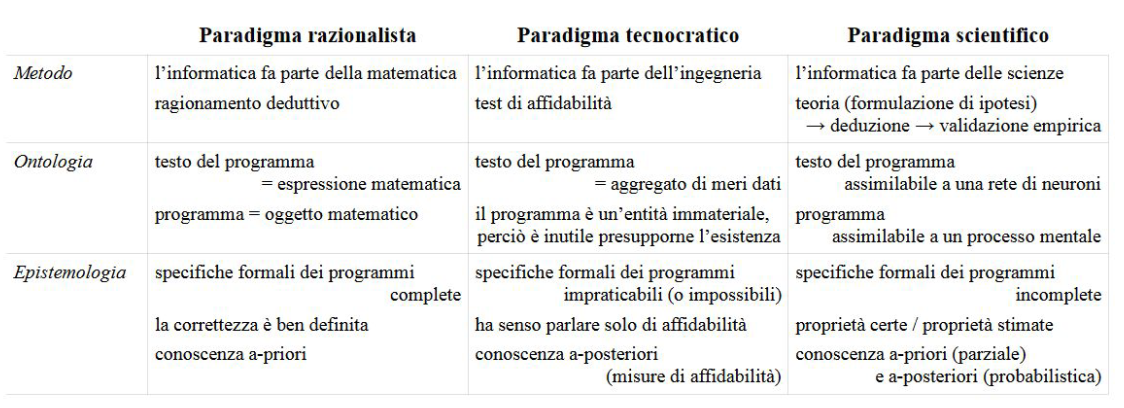
\includegraphics[scale = 0.4]{images/introduzione/Paradigmi.png}
\end{center}


\dfn{Paradigma razionalista (o matematico)}{Per il \newfancyglitter{paradigma razionalista} si  formalizza un linguaggio che garantisce certe proprietà (il tutto prima dell'esecuzione).}

\dfn{Paradigma tecnocratico (o ingegneristico)}{Per il \newfancyglitter{paradigma tecnocratico} si devono fare molti test di affidabilità con diversi input (unit test, a run time).}

\dfn{Paradigma scientifico}{Per il \newfancyglitter{paradigma scientifico} si deve validare empiricamente la correttezza di un programma.}
\subsubsection{}
Ognuno di questi paradigmi può essere usato per offrire una visione differennte dell'informatica:

\begin{itemize}
    \item alcune attività sono principalmente scientifiche: \evidence{algoritmi sperimentali};
    \item alcune attività sono principalmente ingegneristiche: \evidence{design}, \evidence{sviluppo}, etc;
    \item alcune attività sono principalmente matematiche: \evidence{calcolo di complessità}, \evidence{metodi formali}.
\end{itemize}

\paragraph{Perchè è importante pensarci?}

È importante pensare al prioprio modo di vedere l'informatica perchè ciò andrà a in cui si andrà a insegnare. Come si è visto la risposta è che l'informatica contiene in sè un po' di ogni paradigma, ma ci sono parti che possono essere ritenute, personalmente, più importanti.

\dfn{Anima matematica}{Rimanda al razionalismo filosofico. La \glitter{conoscenza pura} è più affidabile dei propri sensi (\glitter{conoscenza a posteriori}). L'unica metodologia accettabile è il ragionamento deduttivo. Il testo di un programma è un'espressione matematica.}

\dfn{Anima ingegneristica}{Rimanda all'empirismo inglese per cui l'esperienza è la base della conoscenza. È impossibile stabilire una conoscenza a priori sui programmi, l'informatica teorica è pura speculazione. Il metodo per valutare la qualità di un programma è il \glitter{testing} (abbinato alla statistica). Il testo di un programma è un aggregato di dati.}

\dfn{Anima scientifica}{Rimanda al metodo scientifico sperimentale. Si effettuano dei test basandosi su delle ipotesi. Il testo di un programma è assimilato a un \glitter{processo biologico} e la sua istanziazione (esecuzione) è assimilata a un \glitter{processo mentale}.}

\ex{Un algoritmo di ordinamento spiegato in una scuola secondaria di secondo grado}{
Un algoritmo di ordinamento può essere presentato in modi diversi a seconda dell'approccio scelto.

\evidence{Domande matematiche:}
\begin{itemize}
    \item L'algoritmo riesce a ordinare qualsiasi sequenza di dati, a prescindere dalla situazione iniziale, con eventuali ripetizioni?
    \item Gli algoritmi sono tutti uguali o ce ne sono di più efficienti?
    \item C'è un limite oltre cui non esiste un algoritmo pù veloce?
\end{itemize}

\evidence{Domande scientifiche:}
\begin{itemize}
    \item Come si possono misurare sperimentalmente i tempi di calcolo e con quale attendibilità?
    \item I tempi confermano i risultati teorici?
    \item Quali aspetti sono generali e quali contingenti?
    \item Quick Sort è sempre meglio di Insertion Sort?
\end{itemize}

\evidence{Domande ingegneristiche:}
\begin{itemize}
    \item È possibile migliorare le prestazioni di un algoritmo?
    \item Come si organizza il processo di sviluppo?
    \item Quali sono le condizioni ottimali?
\end{itemize}

}

\section{Quali sono i criteri per definire una scienza?}

\begin{itemize}
    \item Organizzata per capire, sfruttare e affrontare fenomeni pervasivi;
    \item Include sia processi naturali che artificiali;
    \item Ha un corpo ben strutturato;
    \item C'è un impegno per la scoperta e validazione dei principi;
    \item I risultati ottenuti sono riproducibili;
    \item Si possono falsificare ipotesi e modelli;
    \item Si riescono a fare ipotesi affifdabili, alcune sorprendenti.
\end{itemize}

\chapter{L'informatica a scuola}

\section{L'organizzazione del sistema scolastico italiano}

I gradi di istruzione in Italia sono:
\begin{enumerate}
    \item Scuola dell'infanzia;
    \item Scuola di primo grado (\evidence{ex elementari});
    \item Scuola secondaria di primo grado (\evidence{ex medie});
    \item Scuola secondaria di secondo grado (\evidence{ex superiori});
    \item Formazione superiore (università, master, dottorato).
\end{enumerate}

\subsection{Come si accede all'insegnamento?}

Per diventare docenti è necessario avere:
\begin{itemize}
    \item un titolo di accesso all'insegnamento (Laurea, Diploma, etc.);
    \item  l'\glitter{abilitazione all'insegnamento}.
\end{itemize}
\paragraph{}
Chi possiede solo il primo requisito può essere inserito nelle graduatorie di istituto di III fascia per incarichi di supplenza a \evidence{tempo determinato}\footnote{In realtà i criteri vengono aggiustati in base all'istituto, abbassando i requisiti}.
\paragraph{}
Quando si consegue l'abilitazione si può accedere alle graduatorie di istituto di II fascia e si può partecipare al \newfancyglitter{concorso}.

\nt{Dalle graduatorie dei concorsi, annualmente, si attinge per l'immissione in ruolo a tempo indeterminato.}

\dfn{Titoli di accesso all'insegnamento per la scuola dell'infanzia e primaria}{
Per accedere all'insegnamento per la scuola dell'infanzia e per la scuola primaria i titoli di accesso sono: Laurea in scienze della formazione primaria, Diploma di Istituto Magistrale o Diploma di Liceo Socio-Pedagogico conseguiti entro l'anno scolastico (2001-2002)\footnote{Tutti questi titoli sono anche abilitanti}.
}

\dfn{Titoli di accesso all'insegnamento per la scuola secondaria di I e II grado}{
Per accedere all'insegnamento per la scuola secondaria di I e II grado è necessario avere un determinato tipo di Laurea appartenente a una \evidence{classe di concorso}. In più bisogna acquisire 60 CFU nei settori: antro/psico/pedagogici/metodologico\footnote{Di cui 16 CFU di disciplina}.
}

\section{Cosa si può insegnare con la laurea magistrale in informatica?}

La \evidence{Laurea magistrale in informatica} dà accesso "diretto\footnote{Se si ha l'abilitazione}" alle classi di concorso:

\begin{itemize}
    \item A-41, Scienze e tecnologie informatiche;
    \item A-47, Scienze matematiche applicate.
\end{itemize}
\subsubsection{}

Mentre, prendendo dei crediti extra in altri settori, si può accedere a:

\begin{itemize}
    \item A-26, Matematica;
    \item A-28, Matematica e scienze;
    \item A-40, Scienze e tecnologie elettriche ed elettroniche.
\end{itemize}


\nt{Nelle scuole, per via di carenza di professori, molte cattedre di informatica sono affidate a docenti di matematica. Questo fa si che ci sia una preparazione molto eterogenea a seconda della scuola.}

\dfn{Le indicazioni nazionali}{
Per ogni scuola e per ogni indirizzo sono presenti le \evidence{indicazioni nazionali} in cui si elencano le competenze presupposte in ingresso, gli obiettivi di apprendimento e le competenze attese in uscita. Gli insegnanti devono progettare le loro attività didattiche a partire da queste indicazioni.
}
\chapter{Le teorie dell'apprendimento}

L'impostazione che si dà a un'attività didattica si basa su:

\begin{itemize}
    \item una \fancyglitter{teoria dell'apprendimento};
    \item l'idea, personale, che si ha di che cosa sia la \fancyglitter{conoscenza}.
\end{itemize}

\section{I paradigmi di apprendimento}

\dfn{Teorie dell'apprendimento}{Le \evidence{teorie dell'apprendimento} descrivono come le persone imparano. Esse sono prodotte da psicologia, pedagogia e filosofia.}

\dfn{I paradigmi dell'apprendimento}{I \evidence{paradigmi dell'apprendimento} sono classificazioni delle teorie in base ai loro tratti comuni.}
\subsubsection{}
Principalmente si individuano due macro-categorie:
\begin{itemize}
    \item istruttivismo;
    \item costruttivismo.
\end{itemize}

\section{Comportamentismo}

\dfn{Comportamentismo}{Si vuole modellare un \newfancyglitter{comportamento desiderabile}. L'apprendimento veniva valutato in base ai cambiamenti nel comportamento degli alunni. Gli studenti sono una \newfancyglitter{tabula rasa} che ricevono passivamente le informazioni per ripetizione. Si modella il comportamento tramite \newfancyglitter{rinforzi}\footnote{Punizioni corporali}.
}

\nt{Questo è un approccio istruttivista il cui focus è sulla trasmissione della conoscenza, sulla strutturazione e presentazione dei contenuti, e non sullo studente, che viene visto come un recipiente da riempire.}

\paragraph{Focus:}

\begin{itemize}
    \item Filosoficamente si ritiene vera l'esistenza di una \fancyglitter{realtà oggettiva} che può essere imparata;
    \item La conoscenza è una \fancyglitter{rappresentazione mentale} della realtà;
    \item C'è il presupposto che il mondo e la conoscenza esista anche se nessun essere umano li percepisce;
    \item Il linguaggio è il mezzo di trasporto della conoscenza.
\end{itemize}

\section{Cognitivismo}

\dfn{Cognitivismo}{Il cognitivismo supera l'idea di osservare solo i comportamenti esterni. Si elaborano alcune teorie:
\begin{itemize}
    \item il \newfancyglitter{carico cognitivo} è il carico di lavoro mentale necessario per eseguire un compito;
    \item gli \newfancyglitter{schemi} e i \newfancyglitter{modelli mentali}.
\end{itemize}
}

\nt{Lo scopo dell'educazione è quello di far ricordare e applicare la conoscenza.}

\paragraph{Focus:}

\begin{itemize}
    \item Gli studenti sono degli \fancyglitter{elaboratori di informazione};
    \item Gli insegnanti devono facilitare l'elaborazione.
\end{itemize}

\nt{Questo approccio è ambivalente: può essere sia istruttivista che costruttivista.}

\section{Costruttivismo}

\dfn{Costruttivismo}{Il costruttivismo\footnote{Ideato da Jean Piaget} si basa sullo \newfancyglitter{scetticismo}:
\begin{itemize}
    \item la conoscenza deriva dall'esperienza\footnote{Soggettiva};
    \item non c'è modo di sapere la "vera" verità.
\end{itemize}
}

\nt{
\begin{itemize}
    \item Il concetto di verità è illusorio;
    \item Non si può confrontare la rappresentazione con l'oggetto rappresentato;
    \item Si deve ricorrere alla "viabilità".
\end{itemize}
}

\dfn{Viabilità}{Una conoscenza viene definità \newfancyglitter{viabile} se ha funzionato bene nelle esperienze precedenti.}

\cor{Criteri di viabilità}{
\begin{itemize}
    \item Azioni fisiche: è viabile tutto ciò che porta allo scopo scelto;
    \item Piano concettuale: non ci deve essere contradditorietà o non coerenza logica. 
\end{itemize}
}

\ex{Alcuni metodi di apprendimento}{
\begin{itemize}
    \item Assimilazione: si incorpora un concetto in uno schema già acquisito;
    \item Accomodamento: si modifica la struttura cognitva in relazione a cose nuove.
\end{itemize}
}

\dfn{Apprendimento attivo}{L'\newfancyglitter{apprendimento attivo} è un ampio insieme di metodologie didattiche che coinvolgono gli studenti come parte \newfancyglitter{attiva} dell'apprendimento insieme all'insegnante.}

\dfn{Costruttivismo cognitivo}{Nel \newfancyglitter{costruttivismo cognitivo} lo scopo dell'educazione è quello di permettere agli studenti di creare nuova conoscenza. L'apprendimento è il processo di costruzione del signidìficato. L'insegnante ha solo lo scopo di facilitare la scoperta offrendo le risorse necessarie.}

\cor{}{Lo sviluppo cognitivo è consentito dall'ambiente culturale e l'apprendimento si deve svolgere con l'aiuto altrui. La \evidence{ZPS}\footnote{Zona di sviluppo prossimale} descrive le possibili zone di sviluppo di un bambino:
\begin{itemize}
    \item zona 1 (o zona di sviluppo attuale): lo studente può apprendere da solo;
    \item zona 2/ZPD (o zona di sviluppo prossimale): lo studente può apprendere solo se supportato;
    \item zona 3 (o zona di sviluppo potenziale): lo studente non può ancora apprendere nè da solo nè supportato. 
\end{itemize}
ZPS}

\nt{Un insegnante può agire solo sulla zona 2.}

\dfn{Socio-costruttivismo}{Nel \newfancyglitter{socio-costruttivismo} lo scopo dell'educazione è quello di permettere agli studenti di creare nuova conoscenza insieme. Si dà enfasi sulle relazioni umane.}

\subsection{Didattica costruttivista}

Le moderne teorie sono molto spesso basate sul costruttivismo:

\begin{itemize}
    \item \evidence{active learning}: le pratiche in cui gli studenti svolgono attivamente qualcosa e riflettono;
    \item \evidence{productive failure}: si chiede agli studenti di svolgere problemi mal strutturati o difficili. In seguito si forniscono le conoscenze necessarie;
    \item \evidence{problem-based learning} (PBL): problema realistico;
    \item \evidence{inquiry-based learning}: gli studenti formulano domande, raccolgono dati, li analizzano, provano a spiegarli e creano conoscenza teorica.
\end{itemize}

\nt{Il productive failure funziona una volta sola, quindi va usato come "jolly".}

\paragraph{Caratteristica della didattica costruttivista:}

\begin{itemize}
    \item[$\Rightarrow$] l'apprendimento non avviene attraverso fasi standard;
    \item[$\Rightarrow$] ogni studente deve avere la possibilità di stabilire il proprio percorso;
    \item[$\Rightarrow$] l'insegnante deve indirizzare;
    \item[$\Rightarrow$] le parole e le azioni del docente sono strumenti per apprendere;
    \item[$\Rightarrow$] si dà priorità all'esperienza diretta piuttosto che alla lezione tradizionale.
\end{itemize}

\nt{Ovviamente l'esperienza diretta va gestita dall'insegnante.}

\paragraph{Compiti del docente:}

\begin{itemize}
    \item[$\Rightarrow$] accertare le pre-concezioni degli alunni;
    \item[$\Rightarrow$] far emergere concezioni sbagliate;
    \item[$\Rightarrow$] ristabilire le idee mediante ipotesi e tentativi;
    \item[$\Rightarrow$] far elaborare una nuova interpretazione coerente a quella socialmente condivisa.
\end{itemize}

\section{Costruzionismo}

\dfn{Costruzionismo}{Il \newfancyglitter{costruzionismo} si basa sull'idea costruttivista di strutture di conoscenza. A ciò viene aggiunta l'idea che ciò accade nei contesti in cui si è coinvolti nella costruzione di un'entità (artefatto).}

\nt{Il costruzionismo è stato ideato da Seymour Papert, l'inventore di LOGO.}

\epigraph{\textbf{I ragazzi si avventurano nell'esplorazione di come loro stessi pensano. L'esperienza può essere esaltante: pensare sul pensare trasforma i ragazzi in epistemologi, un'esperienza rara anche per gli adulti.}}{\textit{Seymour Papert}}











\chapter{Progettazione della didattica}

\section{Le fasi, gli snodi e gli indicatori}

Ogni attività didattica può essere costituita da una o più fasi. Ogni fase a sua volta deve essere svolta secondo uno schema:

\begin{enumerate}
    \item \evidence{consegna}: si introduce la descrizione del compito da svolgere. Deve essere progettato per far emergere dubbi e domande agli studenti;
    \item \evidence{svolgimento}: gli studenti devono svolgere l'attività da soli, in coppia o in gruppo. Il compito dell'insegnante è quello di controllare lo svolgimento della consegna e favorire la discussione;
    \item \evidence{discussione}: ogni studente, coppia o gruppo presenta alla classe la propria soluzione e la discute. Il docente deve far emergere le idee dei singoli. Chiunque presenti una critica a una soluzione deve adeguatamente motivarla;
    \item \evidence{conclusione}: la classe deve essere messa allo stesso livello in base a quanto detto nel punto precedente. L'insegnante si occupa di riassumere i risultati ottenuti.
\end{enumerate}

\nt{La divisione di un'attività in fasi è utile per controllare che ogni studente abbia appreso le competenze necessarie.}

\dfn{Snodi}{Gli \newfancyglitter{snodi} sono i passaggi cognitivi per rispondere correttamente alle domande, svolgere un compito o risolvere un problema.}

\ex{Snodi}{
\begin{itemize}
    \item Comprendere come effettuare una determinata azione;
    \item Eseguire un compito;
    \item Trovare un modo per risolvere un problema.
\end{itemize}
}

\nt{Uno snodo \underline{non è} una fase o una sottofase.}

\dfn{Indicatori}{Gli \newfancyglitter{indicatori} servono per "indicare" se uno snodo è stato superato o meno.}

\ex{Indicatori}{
\begin{itemize}
    \item Frasi;
    \item Domande sulla fase appena svolta;
    \item Commenti sull'attività.
\end{itemize}
}

\section{Obiettivi formativi}

\dfn{Obiettivi formativi}{Gli \newfancyglitter{obiettiv formativi} sono ciò che deve rimanere come apprendimento. Alcune attività possono essere funzionali all'apprendimento in sè pur non avendo contenuti da apprendere.}

\nt{Gli obiettivi dell'insegnamento possono essere \underline{diversi} dagli obiettivi dell'attività.}

\paragraph{Obiettivi formativi:}

\begin{itemize}
    \item \evidence{conoscenze} (K): cosa ci si aspetta che l'alunna conosca dopo l'attività;
    \item \evidence{abilità} (A): cosa ci si aspetta che l'alunno abbia imparato a fare;
    \item \evidence{competenze} (C): come ci si aspetta che l'alunno sappia applicare conoscenze e abilità in un ambiente nuovo, per risolvere un problema.
\end{itemize}

\ex{Obiettivi}{

Lo studente è in grado di $<$verbo di azione$>$ + $<$oggetto$>$ + $[<$specifiche$>]$.
\begin{itemize}
    \item[$\Rightarrow$] Verbo: indica la prestazione attesa. Osservabile e misurabile;
    \item[$\Rightarrow$] Oggetto: la conoscenza che deve essere acquisita;
    \item[$\Rightarrow$] Specifiche: specificano condizioni aggiuntive, tempo, precisione con cui la prestazione deve essere eseguita. Sono opzionali.
\end{itemize}

}

\nt{I verbi non sono casuali, ma sono individuati dalla tassonomia di Bloom}

\dfn{Tassonomia di Bloom}{La \newfancyglitter{tassonomia di Bloom} è un modello di classificazione degli obiettivi educativi che si concentra sui processi cognitivi necessari per completare un compito educativo.}

\nt{La tassonomia di Bloom si articola su più livelli in cui, per proseguire, è necessario aver padroneggiato il piano precedente.}

\begin{center}
    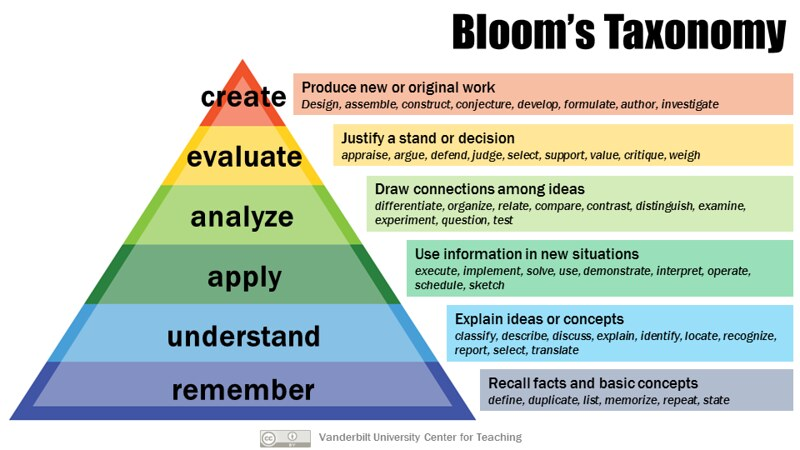
\includegraphics[scale = 0.7]{images/progettazione della didattica/Bloom.jpeg}
\end{center}

\nt{Questa tassonomia va integrata con le indicazioni nazionali, citate in un capitolo precedente.}

\ex{I codici segreti con le vernici}{

\paragraph{Domanda:} come fa un computer a sussurrare il numero di una carta di credito a un altro computer proteggendolo da tutti gli altri computer connessi alla rete?

Per spiegare ciò (lo scambio di chiavi di Diffie-Hellman\footnote{Spiegato in dettaglio nel corso di "Sicurezza"}) si utilizza il trucco delle vernici mescolate:

\begin{itemize}
    \item ognuno ha a disposizione molti colori con nomi precisi;
    \item ognuno ha un set di vernici identico agli altri;
    \item ognuno ha sufficienti barattoli;
    \item ognuno può mescolare le vernici non visto dagli altri.
\end{itemize}

In questo esempio non ci sono comunicazioni segrete, ma solo pubbliche. Il trucco consiste nel fatto che per separare i colori bisogna sapere con quali colori sono formati. Questa è un'attività semplice ma interessante per spiegare il concetto di chiave pubblica e chiave privata.

}







\chapter{Problem solving}

\section{Formulare e comprendere i problemi}

\dfn{Compiti di realtà}{
Negli ultimi anni si fanno svolgere dei \newfancyglitter{compiti di realtà}, ossia dei problemi basati sulla realtà.
}

\dfn{Obblighi impliciti}{
Spesso i bambini tendono a limitarsi pensando a come ci si aspetta che loro debbano rispondere.
}

\ex{Nonna Rosa e la spesa}{

\paragraph{Testo:} Nonna Rosa vuole realizzare una macedonia alla frutta per i suoi nipotini. Le servono 2 kg di albicocche e 3 kg di pesche. Va al mercato per acquistarle. Nel banco della signora Agata (banco A) le pesche costano 1 € al kg e le albicocche 2 € al kg. Nel banco del signor Bruno (banco B) le pesche costano 2 € al kg e le albicocche 1 € al kg. 
Come è più conveniente fare l’acquisto? 
Quanto spenderà  Nonna Rosa?

\paragraph{Risposta semplice:} il procedimento che la maggior parte dei bambini è eseguire il calcolo per il banco A e il calcolo per il banco B e scegliere il banco in cui costa meno.

\paragraph{Risposta creativa:} si prendono le pesche nel banco A e le albicocche nel banco B.

\paragraph{Spiegazione:} solitamente i bambini danno una risposta semplice perchè sono stati abituati al fatto che i problemi vengono posti in un certo modo anche se nel testo non è scritto che si debba scegliere un banco.
}

\nt{È importante pensare al come enunciare i problemi. La formulazione di un problema in quanto tale deve modellare un bisogno reale\footnote{il problema di nonna Rosa insegna che con la matematica si può risparmiare}. Per progettare un compito di realtà bisogna comprendere le possibili interpretazioni dello stesso.}

\ex{Come porre i problemi}{

\paragraph{Formulazione puramente algoritmica:} problemi  che nella formulazione si riferiscono direttamente alle strutture dati e variabili che verranno usate nel programma progettato per risolverli.

\paragraph{Formulazione algoritmico-narrativa:} problemi che  nella formulazione non  si riferiscono esplicitamente alle strutture dati e variabili che verranno usate nel programma progettato per risolverli. La formulazione è inserita in una storia/narrazione. Per risolvere il problema in questo caso si deve prima interpretare il testo. 

\begin{center}
    \begin{tabular}{ | p{3,5cm} | p{4,7cm} | p{5cm} |}
        \hline
        \textbf{Compito}      
    & \textbf{Formulazione puramente algoritmica}
    & \textbf{Formulazione algoritmico-narrativa} \\ \hline\hline
    Trovare il massimo in una lista di numeri
    & Scrivere un programma/algoritmo in pseudo codice che ritorna il numero massimo in una lista di numeri
    & Si svolge una gara di salto in lungo. Trovare l'atleta che ha percorso la distanza maggiore\\ \hline
    
    Dire se un array è ordinato oppure no
    & Scrivere un programma/algoritmo in pseudo codice che ritorna vero se un dato array è ordinato falso altrimenti
    & Si ha un mazzo di carte e si vuole sapere se le carte sono messe in ordine\\ \hline
    
    Crittografare messaggi simulando un cifrario di Cesare
    & Scrivere un programma/algoritmo in pseudo codice che cambi ogni lettera con la sua successiva
    & Dei partner finanziari devono scambiarsi messaggi in codice.  I messaggi possono contenere parole, spazi e punti. Scrivere un metodo che ritorni un messaggio codificato in modo che ogni lettera sia rimpiazzata dalla successiva rispetto all’alfabeto\\
        \hline
        \end{tabular}
    \end{center}

}

\section{I problemi}

\qs{}{Che cos'è un problema?}

\paragraph{Risposta:} un problema è un'entità sconosciuta in qualche situazione. Ovviamente è necessario che ci sia qualcuno interessato a trovare una soluzione.

\nt{La motivazione, specialmente nei compiti di realtà, ricopre un ruolo fondamentale.}

\dfn{Problem solving}{Il \newfancyglitter{problem solving} è una sequenza di attività cognitive orientate a un obiettio unita alla manipolazione dello spazio del problema}

\nt{Un problema ben strutturato:
\begin{itemize}
    \item presenta tutti gli elementi necessari;
    \item richiede l'applicazione di un certo numero di regole e princìpi organizzati in un modo predittivo e prescritto;
    \item presenta soluzioni conoscibili e comprensibili.
\end{itemize}
}

\nt{Un problema non strutturato:
\begin{itemize}
    \item presenta elementi sconosciuti;
    \item ha più soluzioni o nessuna soluzione;
    \item ha più criteri di valutazione;
    \item richiede di esprimere giudizi e opinioni personali.
\end{itemize}
}

\subsection{Complessità dei problemi}

\dfn{Complessità}{
La complessità di un problema è definita da:
\begin{itemize}
    \item numero di aspetti, funzioni o variabili coinvolte;
    \item connettività tra queste proprietà;
    \item relazioni tra proprietà e stabilita nel tempo.
\end{itemize}
}

\nt{Se un problema è mal strutturato si ha una maggior complessità. I problemi ben strutturati coinvolgono un insieme vincolato di variabili prevedibili e comlessità minore.}

\nt{Si ha un problema simile nel corso di "Basi di dati" in fase di progettazione.}





\chapter{Definizione di algoritmo}

\section{Cos'è un algoritmo?}

\nt{Nelle seguenti definizioni si fa implicitamente riferimento al solo paradigma imperativo.}

\dfn{Algoritmo}{
Un \newfancyglitter{algoritmo}: 
\begin{itemize}
    \item necessità di una condizione di terminazione $\rightarrow$ termina sempre;
    \item deve avere chiarezza e precisione nelle istruzioni $\rightarrow$ non si devono lasciare ambiguità.
\end{itemize}
}

\cor{Proprietà di un algoritmo}{
\begin{itemize}
    \item Finitezza: termina in un numero finito di passi;
    \item Precisione: ogni passo è precisamente definito;
    \item I/O: un algoritmo ha 0+ input e ha 1+ output;
    \item Fattibilità: un algoritmo deve essere effettivamente eseguibile;
    \item Correttezza;
    \item Efficienza.
\end{itemize}
}

\nt{In una scuola secondaria bisogna utilizzare un linguaggio più semplice rispetto ai termini accademici. Inoltre per definire un algoritmo o uno pseudo-algoritmo è utile immaginare un'interprete meccanico che deve avere istruzioni per ogni caso possibile.}

\dfn{Problemi computazionali}{Un \newfancyglitter{problema computazionale} è una collezione di domande, le istanze, per cui si sia stabilito un criterio astratto per riconoscere le risposte corrette.}

\ex{Massimo comun divisore}{
Ingressi:
\begin{itemize}
    \item Coppie di interi $a$, $b$ che non siano entrambi nulli. 
\end{itemize}
Uscite:
\begin{itemize}
    \item Un intero $c$ tale che:
    \begin{itemize}
        \item $c$ divide sia $a$ che $b$;
        \item se $d$ divide $a$ e $b$ allora $d$ divide $c$.
    \end{itemize}
\end{itemize}
}
\chapter{Didattica della programmazione}

\section{L'apprendimento}

\nt{I seguenti risultati (teoria dei magazzini di memoria) è frutto degli studi del cognitivismo.}

\begin{center}
    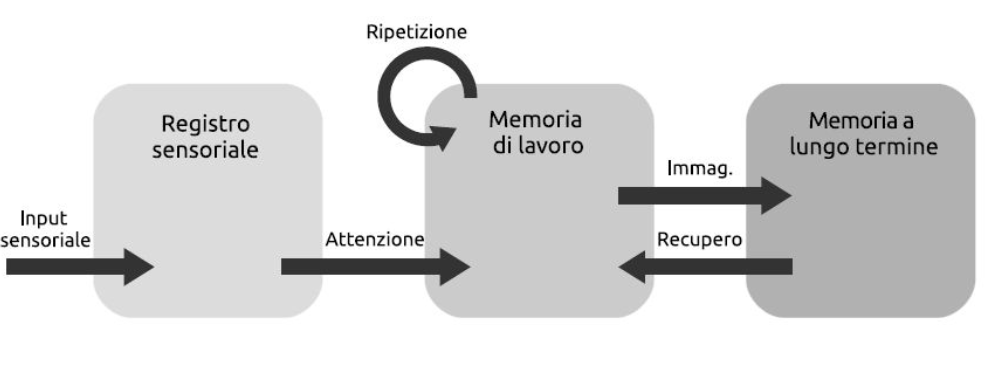
\includegraphics[scale = 0.4]{images/didattica della programmazione/Apprendimento.png}
\end{center}

\dfn{Registro sensoriale}{L'input sensoriale è ciò che viene acquisito dai 5 sensi.}

\nt{Nell'apprendimento l'input è solitamente l'udito o la vista.}

\dfn{Memoria a breve termine (o memoria di lavoro)}{Serve attenzione per passare dal registro sensoriale alla memoria di lavoro. Ha una capienza limitata in termini di spazio e tempo (circa 10 secondi, aumentabli con la ripetizione.}

\nt{Quando si sta imparando la memoria di lavoro è totalmente concentrata su un compito.}

\dfn{Memoria a lungo termine}{Ha capacità potenzialmente illimitate\footnote{Non esattamente}. Non si è coscenti di queste memorie che devono essere portate, ogni volta, nella memoria di lavoro.}

\dfn{Apprendimento}{L'apprendimento richiede che la conoscenza avviene solo quando il concetto passa dalla memoria a breve termine alla memoria a lungo termine.}

\nt{Se si "impara" una cosa, ma il giorno dopo non si riesce più a replicarla non si ha apprendimento.}

\section{La programmazione}

\dfn{Programmare}{La \newfancyglitter{programmazione} è una rappresentazione di base fatta di schemi\footnote{Problemi}, le soluzioni e le informazioni associate.}

\nt{Ciò che distingue un esperto da un principiante è la capacità di attingere a molti più schemi memorizzati nella memoria a lungo termine.}

\qs{}{Com'è possibile che l'uomo riesca a svolgere attività mentali complesse con una memoria di lavoro tanto limitata?}

\begin{itemize}
    \item Si apprende meglio quando la memoria di lavoro non è troppo vuota o troppo piena;
    \item Il carico cognitivo è legato alla memoria di lavoro;
    \item Il carico cognitivo può essere:
    \begin{enumerate}
        \item Intrinseco: imposto dal compito;
        \item Pertinente: usate per creare o modificare schemi, ma non indispensabile;
        \item Estraneo: inutile.
    \end{enumerate}
\end{itemize}

\nt{
\begin{itemize}
    \item Si deve mantenere un carico pertinente elevato;
    \item Se il carico intrinseco è elevato non si apprende\footnote{Ci si concentra sul problema, ma non sugli schemi};
    \item Se il carico cognitivo è basso ci si annoia;
    \item Se possibile conviene ridurre il carico cognitivo di compiti difficili.
\end{itemize}
}

\pagebreak

\section{Pattern}

\ex{Un abuso di pattern}{
\begin{center}
    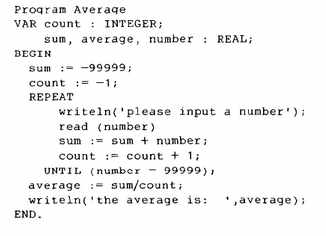
\includegraphics[scale = 0.7]{images/didattica della programmazione/Media.png}
\end{center}

Questo programma è stato scritto da uno studente che aveva intenzione di usare il pattern [Repeat Until] per risolvere il problema della media di una serie di input in cui il valore 99999 funge da guardia. Durante la progettazione lo studente si è trovato con il valore 99999 nella media (che ovviamente non deve essere incluso), motivo per cui ha dovuto inizializzare sum a -99999 (in questo modo i suoi valori si annullano)\footnote{Personalmente la ritengo una soluzione creativa, ma i docenti non sono dello stesso avviso}. Bisogna far capire allo studente che ci sono costrutti più indicati per risolvere questo problema, per esempio il while. Oltre a questo un errore è il count a - 1 che causa una divisione per 0 se si inserisce 99999 all'inizio, ma questo rappresenta un  problema successivo allo studio dei pattern\footnote{Casistica}. 
}

\ex{I pattern}{

\paragraph{Problema:} Si scriva un programma che trovi il minimo in un vettore non ordinato di dimensione nota, maggiore di 0, in cui ogni valore può raggiungere al massimo 99999.

\begin{enumerate}
    \item Input: vettore V[i], dimensione i;
    \item Si inizializza min a 99999, che andrà a trovare il minimo 
    \item Si effettua una [scansione elementare semplice] con l'indice i che viene decrementato a ogni iterazione;
    \item Durante la scansione si effettua una [Guarded-Action];
    \item Se la guardia è soddisfatta si aggiorna la variabile min;
    \item Se la guardia non è soddisfatta si continua finchè il ciclo non termina;
    \item Si stampa il valore min.
\end{enumerate}

}

\dfn{Possibile modo di definire un Pattern algoritmico}{

\begin{center}
    \begin{tabular}{ || p{10cm} ||}
    \hline\hline
    \textbf{Name:} il nome del pattern      
\\ \hline
        \textbf{Initial state:} l'input del programma
        \\
        \textbf{Goal:} l'obiettivo del programma
        \\
        \textbf{Algorithm:} l'algoritmo che risolve il problema
        \\
        \textbf{Remarks:} eventuali osservazioni importanti sul pattern e
        sul suo utilizzo
        \\\hline\hline
    \end{tabular}
\end{center}

}

\cor{Tipi di pattern}{
    \begin{itemize}
        \item [$\Rightarrow$] \textbf{Soluzione a un problema specifico:}
        non costituisce un vero pattern;
        \item [$\Rightarrow$] \textbf{Mezza soluzione - Mezzo pattern:}
        in parte rappresenta un pattern, ma è ancora troppo specifico;
        \item [$\Rightarrow$] \textbf{Quasi pattern:} si può generalizzare,
        ma lo pseudocodice è specifico;
        \item [$\Rightarrow$] \textbf{Pattern:} è generalizzato e lo
        pseudocodice è generico;
        \item [$\Rightarrow$] \textbf{Meta-pattern:} è un pattern che
        descrive un pattern\footnote{Troppo generico.}.
    \end{itemize}
}

\section{Il ruolo delle variabili}

\qs{}{Come viene usata una specifica variabile in un programma? Qual è
il suo ruolo?}

\nt{Si consiglia di non fare un elenco di tutti i vari tipi di utilizzo di
una variabile, ma di presentarli agli studenti quando si devono effettivamente
utilizzare in un programma.}

\dfn{Variabile - Valore fissato}{
    Una variabile assume il ruolo di valore fissato se non verrà mai modificato
    durante l'esecuzione del programma.
}

\nt{Un esempio è il valore di $\pi$.}

\dfn{Variabile - Contatore o indice}{
    Una variabile assume il ruolo di contatore o indice se viene usata per
    scorrere una successione di valori in modo sistematico.
}

\nt{Un esempio è l'indice di un vettore.}

\dfn{Variabile - Valore più recente}{
    Una variabile assume il ruolo di valore più recente se viene usata per
    memorizzare l'ultimo valore letto da un input.
}

\nt{Un esempio è la variabile che memorizza l'ultimo valore letto da un input.}

\dfn{Variabile - Valore più desiderato}{
    Una variabile assume il ruolo di valore più desiderato se viene usata per
    memorizzare il "miglior" valore incontrato fino a quel momento.
}

\nt{Un esempio è la variabile che memorizza il massimo di una successione.}

\subsection{Expert blind spot}

\qs{}{Si è certi che gli studenti siano in grado di riconoscere i ruoli delle variabili?}

\dfn{Expert blind spot}{
    L'expert blind spot è la difficoltà di un esperto di un argomento a
    comprendere le difficoltà che un principiante incontra quando si avvicina
    a quell'argomento.
}

\nt{Ricorda l'effetto Dunning-Kruger.}

\section{Comprensione del codice}

Ricapitolando, programmare vuol dire:

\begin{enumerate}
    \item formalizzare un problema e la sua soluzione;
    \item individuare un procedimento risolutivo;
    \item implementare il procedimento in un linguaggio di programmazione
    in modo che sia eseguibile.
\end{enumerate}

\dfn{Conoscenze}{
    \begin{itemize}
        \item [$\Rightarrow$] \textbf{Conoscenza sintattica:} conoscenza della
        sintassi del linguaggio di programmazione;
        \item [$\Rightarrow$] \textbf{Conoscenza concettuale:} conoscenza di come
        funzionano i costrutti del linguaggio di programmazione;
        \item [$\Rightarrow$] \textbf{Conoscenza strategica:} rappresenta la
        capacità di applicare le precedenti conoscenza per risolvere nuovi
        problemi.  
    \end{itemize}
}

\qs{}{Perchè nei corsi di introduzione alla programmazione si hanno spesso episodi di 
scarsa performance (big failure)?}

\begin{itemize}
    \item [$\Rightarrow$] Scarse competenze di problem solving;
    \item [$\Rightarrow$] Scarsa comprensione dei costrutti necessari per
    programmare;
    \item [$\Rightarrow$] Scarsa capacità di applicare le conoscenze assimilate.
\end{itemize}

\nt{Comprendere il codice e scrivere programmi sono due attività diverse.}

\dfn{Comprensione del codice}{
    La comprensione del codice è il processo cognitivo in cui un individuo costruisce
    una rappresentazione mentale di un programma.
}

\cor{Compito di comprensione del codice}{
    Il compito di comprensione del codice è un'attività tramite la quale si propone
    l'interazione con un pezzo di codice. Tramite questa interazione si costruisce
    una rappresentazione mentale del codice.
}

\mprop{Strategie nella didattica della programmazione}{
    \begin{itemize}
        \item [$\Rightarrow$] Insegnamento esplicito della conoscenza
        strategica;
        \item [$\Rightarrow$] Analisi delle specifiche;
        \item [$\Rightarrow$] Analisi del comportamento del codice; 
        \item [$\Rightarrow$] Tracciatura (simulazione del comportamento del
        programma);
        \item [$\Rightarrow$] Comprensione del codice ("spiega con parole tue");
        \item [$\Rightarrow$] Parsons problems (riordinare le righe di codice);
        \item [$\Rightarrow$] Refactoring di codice;
        \item [$\Rightarrow$] Adattamento di un programma a un compito simile;
        \item [$\Rightarrow$] Completamento di un programma;
        \item [$\Rightarrow$] Debugging;
        \item [$\Rightarrow$] Scrittura di codice.
    \end{itemize}
}

\subsection{Block Model}

\dfn{Block Model}{
    Il Block Model è un framework usato per classificare e analizzare vari aspetti
    della comprensione del codice.
}

\begin{figure}[!h]
    \centering
    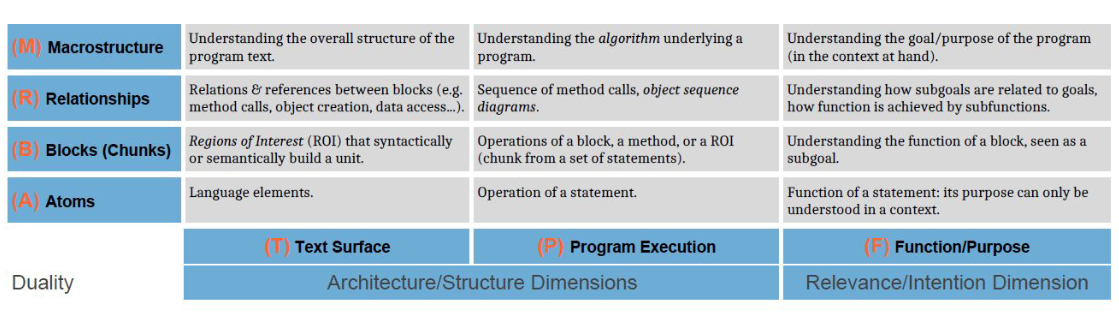
\includegraphics[scale = 0.4]{images/didattica della programmazione/Block Model.png}
    \caption{Block Model}
    \label{fig:my_label}
\end{figure}

\ex{Block Model}{
\begin{center}
    \begin{tabular}{ | p{10cm} | c | c |}
        \hline
        \textbf{\fancyglitter{Esercizio}} & \textbf{\fancyglitter{Comprensione}} & \textbf{\fancyglitter{Strategia}}      
\\ \hline\hline
    Indicare la struttura a blocchi di un programma
    & T
    & M\\\hline
    
    Determinare la presenza di codice ridondante
    & P
    & M\\ \hline
    
    Riassumere un programma in una breve frase
    & F
    & M\\\hline

    Identificare ogni assegnamento nel codice
    & T
    & A\\ \hline
    
    Determinare il valore di una variabile dopo l'esecuzione di un programma
    & P
    & A\\\hline
    
    Spiega lo scopo di un elemento di un programma
    & F
    & A\\ \hline
    
    Identifica lo scopo di una variabile
    & F
    & R\\\hline

    Identifica i blocchi di un programma
    & T
    & B\\ \hline    
    
    Completa il codice e un diagramma di flusso
    & P
    & B\\\hline
    
    Rifletti su un codice
    & T
    & R\\ \hline
    
    Parson's problem
    & P
    & R\\\hline
    
    Spiegare lo scopo di un programma
    & F
    & B\\ \hline
        \end{tabular}
    \end{center}
}

\subsection{Errori degli studenti}

\dfn{I distrattori}{
    I distrattori sono le risposte sbagliate che gli studenti danno più
    frequentemente nei test a risposta multipla. Esse sono impostate
    in modo da corrispondere a specifici errori concettuali.
}

\nt{In questi casi l'insegnate può facilmente individuare cosa lo studente non abbia capito\footnote{Assumendo che lo studente non abbia copiato o tirato a caso.}.}

\cor{5 livelli di risposte}{
    \begin{itemize}
        \item [$\Rightarrow$] \textbf{Prestructural:} la risposta dell'alunno
        è la meno sofisticata tra quelle possibili\footnote{È sintomo
        di un'idea sbagliata o di un preconcetto irrilevante.};
        \item [$\Rightarrow$] \textbf{Unistructural:} la risposta dell'alunno
        mostra una comprensione parziale del problema, una sorta di "congettura
        istruita";
        \item [$\Rightarrow$] \textbf{Multistructural:} la risposta dell'alunno
        rivela una consapevolezza di tutte le parti del problema, ma  non riesce
        a collegarle tra loro\footnote{"Not seeing the forest for the trees".};
        \item [$\Rightarrow$] \textbf{Relational:} la risposta dell'alunno
        rappresenta un'integrazione delle parti del problema;
        \item [$\Rightarrow$] \textbf{Extended abstract:} la risposta dell'alunno va
        al di là del problema immediato ed è collegata a un contesto più ampio;
    \end{itemize}
}

\dfn{Scaffolding}{
    Lo scaffolding è un processo di supporto che aiuta gli studenti:
    \begin{itemize}
        \item Ridurre il carico cognitivo;
        \item Fornire un modello di soluzione adeguato;
        \item Favorire lo sviluppo di una conoscenza strategica.
    \end{itemize}
}

\nt{Ovviamente lo scaffolding deve essere piano piano rimosso.}

\section{Approcci innovativi}

\subsection{PRIMM}

\dfn{PRIMM}{
    PRIMM è un framework per la progettazione di attività didattiche
    per l'insegnamento della programmazione comprendente le seguenti fasi:
    \begin{itemize}
        \item \textbf{Predizione:} gli studenti devono prevedere il
        comportamento di un programma;
        \item \textbf{Esecuzione:} gli studenti devono eseguire il programma
        e verificare la predizione;
        \item \textbf{Investigazione:} gli studenti devono correggere la
        predizione in caso di errore;
        \item \textbf{Modifica:} gli studenti devono modificare il programma
        in modo che si comporti in un modo diverso;
        \item \textbf{Risoluzione:} gli studenti devono risolvere un problema
        usando il programma.
    \end{itemize}

}

\subsection{POGIL}

\dfn{POGIL}{
    POGIL è un framework per la progettazione di attività didattiche
    per l'insegnamento della programmazione. Durante queste attività gli
    studenti attraversano un ciclo di esplorazione, concettualizzazione e
    applicazione.
    Gli studenti scoprono i concetti chiave e costruiscono la propria
    conoscenza attraverso l'interazione con i compagni e con il docente.
}

\subsection{NDL}

\dfn{NDL}{
    NDL (Necessity design learning) è un framework per la progettazione di attività didattiche
    per l'insegnamento della programmazione. Sostanzialmente si dà un problema
    risolvibile con un certo costrutto senza introdurlo. Successivamente,
    prima che lo studente si scoraggi, si introduce il costrutto.
}

\chapter{La natura dei programmi}

\begin{itemize}
    \item [$\Rightarrow$] I programmi sono dappertutto;
    \item [$\Rightarrow$] La programmazione è sempre più presesente nell'ambito scolastico (coding).
\end{itemize}

\section{Che cos'è un programma?}

Questa domanda è molto complicata, la cui risposta cambia a seconda 
della persona a cui la si pone:
\begin{itemize}
    \item se una persona utilizza principalmente applicativi può vedere
    i programmi come strumenti per lavorare, divertirsi, ecc\dots;
    \item se una persona è un programmatore può vedere i programmi come
    una sequenza di istruzioni legata agli algoritmi.
\end{itemize}

\mlenma{}{Fornire agli insegnanti una visione ampia di
cosa sia un programma, al di là di definizioni riduttive o
stereotipate.}

\subsection{Un quadro di riferimento sulla natura dei programmi}

\paragraph{Questo \fancyglitter{framework} può essere utile per:}

\begin{itemize}
    \item capire la \newfancyglitter{centralità dei programmi} ai giorni nostri;
    \item orientare le \newfancyglitter{scelte didattiche}.
\end{itemize}

\paragraph{Il termine \fancyglitter{programma}, in senso lato, è usato:}

\begin{itemize}
    \item dai programmi che si scrivono a scuola ai sistemi operativi.
\end{itemize}

\paragraph{Si considerano solo programmi "\fancyglitter{tradizionali}":}

\begin{itemize}
    \item che implementano \newfancyglitter{algoritmi};
    \item per cui si può \newfancyglitter{spiegare il risultato} ottenuto;
    \item esclusi i programmi prodotti da macchine.
\end{itemize}

\section{Le sfaccettature dei programmi}

\paragraph{I programmi come \fancyglitter{strumenti}:}

\begin{itemize}
    \item [-] utili nel lavoro, nel tempo libero, ecc\dots;
    \item [-] vengono visti come scontati.
\end{itemize}

\paragraph{I programmi come \fancyglitter{opere dell'uomo}:}

\begin{itemize}
    \item [-] sono \textit{solitamente} prodotti con uno scopo preciso;
    \item [-] sono il risultato di scelte.
\end{itemize}

\paragraph{I programmi come \fancyglitter{oggetti fisici}:}

\begin{itemize}
    \item [-] risiedono su un mezzo fisico;
    \item [-] la loro esecuzione richiede tempo ed energia;
    \item [-] hanno bisogno di un dispositivo fisico per essere
    eseguiti.
\end{itemize}

\paragraph{I programmi come \fancyglitter{entità astratte}:}

\begin{itemize}
    \item [-] manipolano nozioni e concetti astratti;
    \item [-] elaborano simboli;
    \item [-] gli effetti fisici sono in funzione del risultato
    astratto;
    \item [-] gli algoritmi sono astratti.
\end{itemize}

\paragraph{I programmi come \fancyglitter{entità eseguibili}:}

\begin{itemize}
    \item [-] sono eseguiti da un calcolatore;
    \item [-] possono essere ripetuti;
    \item [-] l'esecutore è un agente che elabora segnali.
\end{itemize}

\paragraph{I programmi come \fancyglitter{manufatti linguistico-notazionali}:}

\begin{itemize}
    \item [-] rispettano una specifica sintassi;
    \item [-] sono un modo per esprimere idee;
    \item [-] sono un modo per comunicare idee;
    \item [-] possono essere tradotti in altre notazioni.
\end{itemize}

\nt{I programmi sono scritti da persone per essere compresi da altre
persone e per essere eseguiti da una macchina che non li comprende.}



\chapter{Cenni sulla valutazione dell'apprendimento}

Una rubrica \glitter{valutativa} non serve solamente per assegnare un voto a uno studente,
ma anche per \newfancyglitter{aiutarlo a capire} quali sono i suoi punti di \fancyglitter{forza} e di \fancyglitter{debolezza} per poter migliorare.

\nt{Lo studente deve essere parte attivà del processo di valutazione.}

\section{Conoscenze, abilità e competenze}

\dfn{Conoscenze}{
    Le \newfancyglitter{conoscenze} indicano i risultati delle informazioni assimilate.
}

\nt{Le conoscenze sono descritte come teoriche e/o pratiche.}

\dfn{Abilità}{
    Le \newfancyglitter{abilità} indicano la capacità di applicare le conoscenze.
}

\nt{Le abilità sono descritte come cognitive (uso del pensiero logico) e pratiche
(che richiedono l'uso di materiali).}

\dfn{Competenze}{
    Le \newfancyglitter{competenze} indicano la capacità di applicare le conoscenze e le abilità in un contesto specifico.
}

\nt{Le competenze sono descritte in termini di responsabilità e autonomia.}
\afterpage{\blankpage}
\chapter{Letture}

\section{\href{https://dighum.ec.tuwien.ac.at/wp-content/uploads/2019/07/Vienna_Manifesto_on_Digital_Humanism_IT.pdf}{Manifesto di vienna per l'umanesimo digitale}}

\paragraph{Il sistema sta fallendo.} Tim Berners-Lee\footnote{Il fondatore del web} sostiene che la digitalizzazione porti con sè vari problemi: perdità di \evidence{privacy}, insorgere di \evidence{comportamenti estremisti}, formazione di \evidence{bolle informative}, etc. Per sostenere l'\glitter{innovazione tecnologica} c'è bisogno di un vasto \glitter{impegno sociale}.

\paragraph{Il manifesto.} Si rivolge alle comunità \evidence{accademiche} e \evidence{professionali}, ai leader \evidence{industriali} e \evidence{politici}.

\paragraph{Tecnologia e società.} I recenti sviluppi tecnologici \newfancyglitter{creano} e \newfancyglitter{distruggono} posti di lavoro e ricchezza. Viene modificata la gerarchia tra \newfancyglitter{uomo} e \newfancyglitter{macchina}.

\paragraph{L'approccio illuminista e umanista.} Il manifesto rappresenta un'estensione della tradizione intellettuale dell'\evidence{umanesimo} che ambisce a creare un'umanità \evidence{illuminata}.

\paragraph{Le tecnologie digitali.} Esse nascono da scelte \glitter{implicite} ed \glitter{esplicite} che promuovono valori, norme, interessi economici, etc.

\paragraph{Umanesimo digitale.} Si deve spostare il \newfancyglitter{focus} dalle tecnologie all'uomo.

\paragraph{I \evidence{princìpi fondamentali} sono:}

\begin{itemize}
    \item Le tecnologie digitali dovrebbero essere progettate per promuovere \\la democrazia
e l‘inclusione;
\item La privacy e la libertà di parola sono valori essenziali per la democrazia e dovrebbero
essere al centro delle nostre attività;
\item Devono essere stabilite norme, regole e leggi efficaci, basate sul dibattito pubblico
e su un ampio consenso;
\item I regolatori devono intervenire sui monopòli tecnologici;
\item Decisioni le cui conseguenze possono influire sui diritti umani individuali o collettivi
devono continuare a essere prese dalle persone;
\item Approcci scientifici interdisciplinari sono un prerequisito per affrontare le sfide
future;
\item Le università sono il luogo in cui si producono nuove conoscenze e si coltiva
il pensiero critico;
\item I ricercatori accademici e industriali devono aprirsi al dialogo con la società e valutare
criticamente i propri approcci;
\item I professionisti di tutto il mondo dovrebbero riconoscere la loro corresponsabilità
nell‘impatto sociale delle tecnologie digitali;
\item È necessaria una visione che consideri nuovi programmi di studio che combinino
la conoscenza delle scienze umane e sociali e degli studi scientifico-ingegneristici;
\item L‘educazione all‘informatica e al suo impatto sociale devono iniziare il prima
possibile.
\end{itemize}

\section{\href{https://link-and-think.blogspot.com/2019/02/informatica-la-terza-rivoluzione-dei-rapporti-di-potere.html}{Informatica: la terza rivoluzione "dei rapporti di potere"}}

L'\evidence{informatica} è una vera e propria rivoluzione per la razza umana, la terza dopo quella della \newfancyglitter{stampa} e quella \newfancyglitter{industriale}.

L'invenzione della stampa nel XV secolo è stata una rivoluzione sia di tipo \evidence{tecnico}\footnote{Si producono testi più velocemente e più economicamente} che di tipo \evidence{sociale}\footnote{Favorisce una maggiore diffusione della conoscenza}. Il potere della \glitter{conoscenza} non è più confinato alle persone che lo posseggono, perchè ogni testo può essere \newfancyglitter{replicato}. La diffusione di testi scientifici, giuridici e letterari hanno portato la società a essere più \evidence{democratica}.

Ed è proprio la conoscenza scientifica\footnote{In primis il metodo Galileiano} a portare alla rivoluzione industriale. A partire dal '700 la disponibilità di \evidence{macchine} rende possibile l'\newfancyglitter{automatizzazione} del lavoro fisico delle persone. Questa rivoluzione ha carattere \evidence{tecnico} perchè permette di ricreare velocemente i manufatti. Inoltre le macchine non si stancano, quindi possono lavorare giorno e notte. Questo mette in discussione il potere della \evidence{natura}: l'uomo la assoggetta e ne superà i limiti.

Nella seconda metà del '900 inizia la terza grande rivoluzione: l'informatica. Essa non è più una replica della conoscenza statica dei libri o della forza fisica delle persone, ma è "\evidence{conoscenza in azione}". Il sapere non è una rappresentazione \newfancyglitter{statica} dei fatti, ma uno scambio di dati \newfancyglitter{interattivo} tra soggetto e realtà. Il potere che viene minato è l'\evidence{intelligenza umana}: essa può essere in qualche modo replicata dai programmi. Basti pensare agli scacchi in cui il computer è in grado di battere un campione del mondo. Oppure ai recenti sviluppi dell'\evidence{intelligenza artificiale}. Tuttavia ci sono due cose che le "macchine cognitive" non sono ancora riuscite a emulare: la \glitter{flessibilità} e l'\glitter{adattabilità}.

In conclusione: è inevitabile il diffondersi di queste nuove tecnologie e dei cambiamenti a loro collegati, ma è importante che ogni individuo sia istruito e formato sulle basi concettuali che permettono di costruire queste macchine.

\pagebreak


\section{\href{https://link-and-think.blogspot.com/2019/03/informatica-e-competenze-digitali-cosa.html}{Informatica e competenze digitali: cosa insegnare?}}

\paragraph{Risposta breve:} entrambe.

\paragraph{Risposta lunga:} questo intero articolo.
\paragraph{}
Nel mondo scolastico c'è confusione tra i termini "\evidence{informatiche}" e "\evidence{digitali}". Purtroppo negli ultimi 30 anni si sono usati in modo intercambiabile questi due termini per riferirsi a: programmare in Pascal, usare Word, scrivere e-mail,  coding, usare i social, etc.

Digitale si riferisce alla rappresentazione di un dato con un simbolo numerico. Informatico si riferisce alla capacità di \evidence{elaborazione automatica} dei dati resa possibile dai metodi e dalle teorie dell'informatica. Usare dei simboli numerici non è una novità, ma lo è elaborare le informazioni in modo automatico, come se si usasse un gigantesco \evidence{orologio}.

L'orologio è solo un esecutore meccanico che non sa che cosa rappresenta o come sia costruito. Il computer quindi può manipolare simboli e istruzione che per lui non hanno significato, ma che lo hanno per l'uomo. Questo è ala base della terza rivoluzione "dei rapporti di potere".

C'è ancora confusione anche sui documenti ufficiali dell'unione europea in cui, per esempio, la programmazione rientrà tra le competenze digitali, sebbene non lo sia. Negli USA o in UK è una competenza informatica. In questi paesi, l'attuale società è semplicemente un'estensione della società \evidence{industriale}. Infatti la società \evidence{digitale} utilizza delle macchine\footnote{Di tipo cognitivo, non meccanico}. Per trasmettere la comprensione della società digitale è necessario portare nelle scuole l'informatica. Ciò non nega l'insegnamento delle competenze digitali che occupano un ruolo chiave nella condivisione della conoscenza.
\chapter{Domande e risposte}

\section{La natura dell'informatica}

\qs{}{Quali sono i problemi dell'informatica?}

\sol{il termine "informatica" è spesso utilizzato in modo improprio nel linguaggio comune. 
per esempio, viene usato per riferirsi a computers, cellulari, televisori, etc. Ma l'informatica non rigurda
i computers che sono solo uno strumento, non il fine. Un altro problema è il termine "digitale" che, solitamente, 
viene usato come sinonimo di "informatica". In realtà, digitale si riferisce alla rappresentazione di un dato 
mediante un simbolo numerico e a tutte le tecnologie basate sui computers.}

\qs{}{Quali sono i problemi relativi all'insegnamento dell'informatica nel nostro sistema scolastico?}

\sol{l'informatica viene spesso trattata come una non-materia, per cui 
chiunque sappia usare un banale applicativo come Word o Excel tende a comportarsi
come un esperto (si è vista in precedenza la distinzione tra informatico e digitale).
Inoltre un problema endemico della scuola italiana riguarda la carenza di informatici
che insegnino la materia, infatti spesso si ricorre a docenti di matematica (
    la cui classe di concorso li rende "idonei" a insegnare informatica).
}

\qs{}{Perchè è importante insegnare informatica fin dalla scuola primaria?}

\sol{Come le scienze naturali (di cui fa parte) l'informatica offre una chiave di
lettura del mondo che ci circonda, per cui è opportuno iniziare a studiarla il prima possibile
e che ogni studente ne abbia una conoscenza di base. Inoltre, l'informatica è una materia
che si presta molto bene a essere insegnata in modo interdisciplinare.}

\qs{}{Perchè è importante riflettere sulla natura dell'informatica prima di insegnarla?}

\sol{perchè ciò andrà a impattare sul modo di insegnare la materia. A seconda della propria visione del
mondo si privilegeranno alcuni aspetti rispetto ad altri. Inoltre bisogna sempre chiedersi il perchè si studia informatica:
essa dà una chiave di lettura del mondo digitale che è sempre più presente nella nostra quotidianità.}
\pagebreak
\qs{}{Quali sono le 3 anime/paradigmi che abbiamo discusso per inquadrare la natura dell'informatica?}

\sol{

\begin{itemize}
    \item matematico: l'informatica vista come una scienza matematica che formalizza i problemi e li risolve mediante algoritmi;
    \item ingegneristico: l'informatica vista come un'ingegneria che si occupa di progettare e realizzare sistemi software; 
    \item scientifico: l'informatica vista come una scienza che studia i sistemi software e i processi di sviluppo empiricamente.
\end{itemize}
}
\section{Teorie dell'apprendimento}

\qs{}{Che cos'è il comportamentismo?}

\sol{il comportamentismo è una teoria dell'apprendimento che si basa sull'osservazione del comportamento. Essa prevede
di modellare un comportamento desiderabile. La valutazione si basa sui cambiamenti nei comportamenti degli alunni visti come "tabule rase".
Spesso erano previsti "rinforzi" ossia punizioni corporali. Questo approccio è istruttivista.}

\qs{}{Che cos'è il cognitivismo?}

\sol{il cognitivismo rappresenta un superamento del comportamentismo. Il cognitivismo è una teoria dell'apprendimento che si basa
su alcune idee principali:
\begin{itemize}
    \item il carico cognitivo: il carico di lavoro mentale che un individuo deve sostenere per svolgere un compito;
    \item gli schemi e i modelli mentali.
\end{itemize}

L'approccio cognitivista punta a far ricordare e applicare la conoscenza.
}
\qs{}{Che cos'è il costruttivismo? (socio-costruttivismo e costruttivismo cognitivo)}

\sol{ il costruttivismo (ideato da J. Piaget) è una teoria dell'apprendimento che si basa sullo scetticismo:
\begin{itemize}
    \item la conoscenza è frutto dell'esperienza;
    \item non c'è modo di sapere la "vera" verità.
\end{itemize}

\paragraph{Si ricorre alla "viabilità" per valutare la conoscenza:} un'idea è valida se ha funzionato fino a quel momento. Per le azioni fisiche è viabile tutto ciò che
porta a un risultato. Sul piano concettuale ci si basa sulla non contradditorietà.

\begin{itemize}
    \item [$\Rightarrow$] Socio-costruttivismo: l'apprendimento è un processo sociale che avviene in un contesto sociale. Si crea insieme nuova conoscenza;
    \item [$\Rightarrow$] Costruttivismo cognitivo: l'apprendimento è il processo di costruzione del significato. L'insegnante deve solo facilitare la scoperta
    offrendo le risorse necessarie.
\end{itemize}
}
\qs{}{Che cos'è il costruzionismo?}

\sol{il costruzionismo (ideato da S. Papert) si basa sull'idea costruttivista di conoscenza. Ma a ciò viene aggiunta l'idea che la conoscenza deve essere
finalizzata alla costruzione di artefatti.}

\qs{}{Quali sono i punti fondamentali del brano di Papert "Gli ingranaggi della mia infanzia"?}

\sol{}

\begin{itemize}
    \item è più facile apprendere qualcosa se lo si assimila a modelli
    già posseduti (per Papert gli ingranaggi e il differenziale);
    \item al contrario l'apprendimento è più ostico se non si ha un modello
    di riferimento;
    \item oltre agli aspetti cognitivi, l'apprendimento è influenzato da
    aspetti emotivi;
    \item gli ingranaggi sono un qualcosa di personale per Papert, non
    funzionerebbero come modello per tutti.
\end{itemize}

\qs{}{Cos'è l'assimilazione?}

\sol{l'assimilazione è l'incorporazione di un determinato concetto in uno schema che è stato già acquisito.}

\qs{}{Cos'è l'accomodamento?}

\sol{l'accomodamento è la modifica di una struttura cognitiva in relazione al contatto con nuove informazioni.}

\qs{}{Cos'è la zona di sviluppo prossimo (ZSP)?}

\sol{la zona di sviluppo prossimo è la seconda delle tre aree di apprendimento di un bambino. Nella ZSP il bambino è in grado di apprendere solo con il supporto del docente ed è in quest'area che l'insegnante può intervenire.}

\qs{}{Quali sono le caratteristiche principali dell'apprendimento attivo?}

\sol{l'apprendimento attivo nasce dalla didattica costruttivista.}

\begin{itemize}
    \item l'apprendimento non avvene attraverso fasi standard;
    \item ogni studente ha la possibilità di stabilire il proprio percorso;
    \item l'insegnante è un facilitatore;
    \item le parole e le azioni del docente sono strumenti per apprendere;
    \item si dà la priorità all'esperienza diretta (gestita dall'insegnente).
\end{itemize}

\section{Problemi, compiti, spazio di rappresentazione del problema}

\qs{}{Descrvere la differenza tra compito, problema ben/mal strutturato, formulazione narrativa e algoritmica di un problema.}

\sol{}

\begin{itemize}
    \item compito: è un'entità sconosciuta in qualche situazione, per cui è necessario trovare una soluzione.
    Può essere presentato sotto forma di "compito di realtà", ossia basato su 
    eventi verosimili;  
    \item problema ben strutturato: è un problema che presenta tutti gli elementi necessari
    alla risoluzione, richiede l'applicazione di regole e princìpi organizzati in modo 
    predittivo e prescrittivo, ha una soluzione conoscibile e comprensibile;
    \item problema mal strutturato: è un problema che presenta elementi sconosciuti,
    ha più soluzioni o nessuna soluzione, ha più criteri di valutazione, richiede di esprimere
    giudizi e valutazioni;
    \item formulazione narrativa: è una descrizione del problema in linguaggio naturale
    che racconta qualcosa;
    \item formulazione algoritmica: è una descrizione del problema in linguaggio formale
    riferendosi direttamente alle strutture dati e alle variabili richieste.
\end{itemize}

\qs{}{Spiegare il ruolo e l'importanza della rappresentazione e manipolazione dello spazio del problema come parte delle strategie di problem solving.}

\sol{È importante che i problemi siano simulazioni di problemi quotidiani e 
professionali, in cui l'insegnante abbia scelto che componenti includere e come
rappresentarle. Se il problema è ben strutturato, la rappresentazione dello spazio
è semplice per via del modo prevedibile in cui si comportano le variabili,
quindi è, generalmente, più semplice. Viceversa con un problema mal strutturato
la rappresentazione dello spazio è più complessa e richiede più tempo.}

\section{Struttura dell'esame}

\begin{enumerate}
    \item \textbf{Discussione dell'attività didattica (40\% del voto):} i membri del gruppo
    presentano il lavoro svolto e rispondono a eventuali domande;
    \item \textbf{Discussione delle consegne (30\% del voto):} si devono discutere alcune delle consegne svolte.
    In questa parte si può guardare ciò che si è scritto;
    \item \textbf{Domande (30\% del voto):} vengono poste domande sul corso\footnote{Presenti in questa sezione.}. 
\end{enumerate}

\nt{Se si svolge in gruppi ricordare:
\begin{itemize}
    \item di parlare in maniera omogenea, si raccomanda di prepararsi ognuno 
    una propria parte e di non improvvisare;
    \item che ogni membro deve comunque sapere tutto dell'attività;
    \item che la discussione sulle consegne è individuale.
\end{itemize}
}

\end{document}